\documentclass[12pt,paper=a4]{report}
\usepackage{fontspec}
\usepackage{xunicode}
\usepackage{xltxtra}
\usepackage{polyglossia}
\setdefaultlanguage{latvian}
\usepackage{fixlatvian}
\usepackage{caption}
\usepackage{amsmath}
\usepackage{algorithm}
\usepackage[noend]{algpseudocode}
\usepackage{listings}
\usepackage{tocloft}
\usepackage{float}

\makeatletter
\def\BState{\State\hskip-\ALG@thistlm}
\makeatother
\newcommand\var{\texttt}
\interfootnotelinepenalty=10000
\setotherlanguages{english,russian,french}
\setmainfont[Mapping=tex-text]{Times New Roman}%{LMRoman10}
% Fonts krievu valodai, kurā ir arī krievu valodas burti
\newfontfamily\russianfont{Times New Roman}
% Šos fontus tālāk izmantos chapter virsrakstos un url'os (lai būtu kirilicas burti)
\newfontfamily\sffamily{Verdana}
\captionsetup{justification=centering}
\usepackage{setspace}
\newcommand{\nocontentsline}[3]{}
\newcommand{\tocless}[2]{\bgroup\let\addcontentsline=\nocontentsline#1{#2}\egroup}
% lai varam normāli rakstīt apakšvītras
\usepackage{underscore}
% Lai varam iekļaut attēlus
\usepackage{graphicx}
% Kurā vietā tiks meklēti attēli - relatīvais ceļs attiecībā pret dokumentu
\graphicspath{{./PNG/}{./images/internet/}{./images/self-generated/}}
% Ar šiem PDF'ā būs saliktas saites un tām va uzlikt krāsu
\usepackage{hyperref}
\hypersetup{ colorlinks, citecolor=black, filecolor=black,linkcolor=black,urlcolor=black }

\usepackage{amsmath}
\usepackage{amsfonts}
\usepackage{lipsum} %Lai ģenerētu nejaušus tekstus...
\usepackage{listingsutf8}
\usepackage{xcolor}

%\usepackage{inconsolata}
\lstset{
    language=bash, %% Troque para PHP, C, Java, etc... bash é o padrão
    basicstyle=\small,
    numberstyle=\small,
    numbers=left,
    backgroundcolor=\color{gray!10},
    frame=single,
    tabsize=2,
    rulecolor=\color{black!30},
    title=\lstname,
    escapeinside={\%*}{*)},
    breaklines=true,
    breakatwhitespace=true,
    framextopmargin=1pt,
    framexbottommargin=1pt,
    extendedchars=false,
    inputencoding=utf8
}

\usepackage{titlesec}
\titleformat{\chapter}{\huge\centering\sffamily}{\thechapter}{1pc}{}

\addto\captionslatvian{
\renewcommand\bibname{Izmantotās literatūras un avotu saraksts}
}
\clubpenalty10000
\widowpenalty10000
\setlength{\topmargin}{0cm}
\setlength{\headheight}{0in}
\setlength{\headsep}{0in}
\setlength{\textheight}{22.7cm}
\setlength{\textwidth}{15cm}
\setlength{\oddsidemargin}{0.5in}
\setlength{\evensidemargin}{0.5in}
\usepackage{indentfirst}
\hyphenpenalty=5000
\usepackage{totcount}
\newcounter{nofappendices}
\setcounter{nofappendices}{0}
\regtotcounter{nofappendices}
\newtotcounter{fignum}
\def\oldfigure{} \let\oldfigure=\figure
\def\figure{\stepcounter{fignum}\oldfigure}
\newtotcounter{citnum}
\def\oldbibitem{} \let\oldbibitem=\bibitem
\def\bibitem{\stepcounter{citnum}\oldbibitem}
%% Sarakstam visus mainīgos
%% Mainīgie titullapai, defAutors tiek izmantots arī galvojumā
\def\defAutors{Edgars Skore}
\def\defAugstskola{Ventspils Augstskola}{\fontfamily{russianfont}
\def\defFakultate{Informācijas tehnoloģiju fakultāte}
\def\defSProgrammas{dabas zinātņu maģistra studiju programmas\\
	      datorzinātnēs}
\def\defStudents{2. kursa students \\
	      \defAutors}
\def\defMatrikulasNr{16080002}
\def\defDarbaNosaukums{Cilvēku plūsmas analīze, pielietojot konvolūcijas tīklus}
\def\defDarbaNosaukumsEN{Human flow analysis using Convolutional Neural Networks}
\def\defDarbaNosaukumsFR{La grande question sur la vie, l'univers et le reste}
\def\defDarbaNosaukumsLV{Pagātnes, tagadnes un nākotnes aspekti atbildei uz galveno jautājumu}
\def\defDarbaNosaukumsRU{Ответ на главный вопрос жизни, вселенной и всего такого}
\def\defDarbaVeids{Maģistra darbs}
\def\defFakultatesDekans{doc.  Dr.phys. M.~Ēlerts}
\def\defZinVaditajs{Dr.sc.comp. Gundars Bergmanis-Korāts}
\def\defGads{2018}

\usepackage{lipsum}

\def\abstract{

\vspace*{-4\baselineskip}
	\chapter*{\begin{center} \abstractname \end{center} } % start chapter
	\vspace*{-2.5\baselineskip}
  \addcontentsline{toc}{chapter}{\abstractname} % table of contents line
  \markboth{\MakeUppercase{\abstractname}}{} % header mark
  \thispagestyle{empty}
}
\def\endabstract{}%\clearpage
\newenvironment{absolutelynopagebreak}
{\par\nobreak\vfil\penalty0\vfilneg
	\vtop\bgroup}
{\par\xdef\tpd{\the\prevdepth}\egroup
	\prevdepth=\tpd}
\begin{document}

%%%% Titullapas sākums
\begin{titlepage}
\begin{center}
\textsc{
\defAugstskola\\
\defFakultate}\\
\vspace{2em}
\textbf{\defDarbaVeids}\\
\vspace{2em}
{\LARGE \textbf{\defDarbaNosaukums}}\\
\vspace{2em}
\begin{tabular}{@{}r@{}l@{}}
\parbox[c]{0.4\textwidth}{Autors:}&
\parbox[t]{0.6\textwidth}{
\defAugstskola s\\
\defFakultate s\\
\defSProgrammas\\
\defStudents \\
Matrikulas~Nr. \defMatrikulasNr\vspace{0.7em}\\
\mbox{}\hrulefill\vspace{-0.4em}\\
{\scriptsize(paraksts)}\vspace{2em}} \\
\parbox[c]{0.4\textwidth}{Fakultātes dekāns:}&
\parbox[t]{0.6\textwidth}{
\defFakultatesDekans\vspace{.7em}\\
\mbox{}\hrulefill\vspace{-0.4em}\\
{\scriptsize(paraksts)}\vspace{2em}} \\
\parbox[c]{0.4\textwidth}{Zinātniskais vadītājs:}&
\parbox[t]{0.6\textwidth}{
\defZinVaditajs\vspace{.7em}\\
\mbox{}\hrulefill\vspace{-0.4em}\\
{\scriptsize(paraksts)}\vspace{2em}} \\
\parbox[c]{0.4\textwidth}{Recenzents:} & \vspace{.7em}\\
\multicolumn{2}{@{}c@{}}{
\mbox{}\hrulefill
}\vspace{-0.4em}\\
\multicolumn{2}{@{}l@{}}{
{\scriptsize(Ieņemamais amats, zinātn. nosaukums,
vārds, uzvārds)}
}\vspace{.7em}\\
&\mbox{}\hrulefill\vspace{-0.4em}\\
&{\scriptsize(paraksts)}\\
\end{tabular}
\vfill
Ventspils, \defGads
\end{center}
\end{titlepage}
\onehalfspace
\begin{absolutelynopagebreak}
{
	\selectlanguage{latvian}
	\begin{abstract}
		
		\begin{tabular}{@{}r@{}l@{}}
			\parbox[c]{0.3\textwidth}{\textbf{Darba nosaukums:}}&
			\parbox[t]{0.65\textwidth}{\defDarbaNosaukums} \\
			\parbox[c]{0.3\textwidth}{\textbf{Darba autors:}}&
			\parbox[t]{0.65\textwidth}{\defAutors} \\
			\parbox[c]{0.3\textwidth}{\textbf{Zinātniskais vadītājs:}}&
			\parbox[t]{0.65\textwidth}{\defZinVaditajs} \\
			\parbox[c]{0.3\textwidth}{\textbf{Darba apjoms:}}&
			\parbox[t]{0.65\textwidth}{\textcolor{black}{\pageref{LastPage}} lapas, 4 tabulas,  \total{fignum}~attēli, 5 vienādojumi, \total{citnum}~literatūras avoti, 4 pielikumi} \\
			\parbox[c]{0.3\textwidth}{\textbf{Atslēgas vārdi:}}&
			\parbox[t]{0.65\textwidth}{ Datorredze, Dziļā mašīnmācīšanās, Konvolūcijas neironu tīkli, Objektu detektēšana, Objektu sekošana} \\
			&\\
		\end{tabular}

Cilvēku plūsmas analīze ir metožu kopums, kas sniedz iespēju no video datiem izgūt informāciju par cilvēku pārvietošanos konkrētā vietā. Pētniecības darba mērķis ir izstrādāt risinājumu, kas ļauj veikt cilvēku plūsmas analīzi, izmantojot konvolūcijas tīklu cilvēku noteikšanai un sekošanas algoritmus cilvēku izsekošanai video. Pirms risinājuma izveidošanas tika apskatītas eksistējošās plūsmas analīzes metodes, apskatīti un salīdzināti dažādas konvolūcijas neironu tīklu arhitektūras, objektu detektēšanas algoritmi un sekošanas algoritmi.

Plūsmas analīzes algoritma implementācija tika veidota programmēšanas valodā \textit{Python}, izmantojot \textit{caffe} un \textit{darknet} ietvarus. Tika salīdzinātas abu minēto ietvaru piedāvātās \textit{SSD} un \textit{YOLO} objektu detektēšanas algoritmu implementācijas. Tika implementēti objektu sekošanas algoritmi, balstoties uz minēto detektēšanas sistēmu atgrieztajiem rezultātiem.

Pēc plūsmas analīzes risinājuma izstrādes un rezultātu izvērtēšanas, var secināt, ka, praktiski implementētie sekošanas algoritmi nespēj atrast objektus, kad tie pazūd aiz priekšplānā esošajiem objektiem. Izmantojot video fragmentus, kas filmēti no paaugstināta skatu punkta, tādējādi samazinot iespēju objektiem pārklāties, darba ietvaros izstrādātais risinājums veiksmīgi darbotos.
	\end{abstract}
}
\end{absolutelynopagebreak}
%%%% 1.5 līiniju atstarpe starp rindām
\onehalfspace
{
\selectlanguage{english}
\begin{abstract}

\begin{tabular}{@{}r@{}l@{}}
\parbox[c]{0.3\textwidth}{\textbf{The title:}}&
\parbox[t]{0.65\textwidth}{\defDarbaNosaukumsEN} \\
\parbox[c]{0.3\textwidth}{\textbf{Author:}}&
\parbox[t]{0.65\textwidth}{\defAutors} \\
\parbox[c]{0.3\textwidth}{\textbf{Academic Advisor:}}&
\parbox[t]{0.65\textwidth}{\defZinVaditajs} \\
\parbox[c]{0.3\textwidth}{\textbf{The volume of the work:}}&
\parbox[t]{0.65\textwidth}{\textcolor{black}{\pageref{LastPage}} pages, 4 tables,  \total{fignum}~images, 5 equations, \total{citnum}~literature sources, 4 appendices} \\
\parbox[c]{0.3\textwidth}{\textbf{Keywords:}}&
\parbox[t]{0.65\textwidth}{ Computer vision, Deep learning, Convolutional neural networks, Object detection, Object tracking} \\
&\\
\end{tabular}
%\total{nofimages} % ja nu gadiijumaa vajag custom counter

Human flow analysis is a set of methods that, by using video processing, allows us to make conclusions of people movement. The aim of the paper was to create a solution that would allow analyzing human flow by using convolutional network for human detection and tracking algorithms for human tracking. Before coming up with the solution, the Author observed existing methods of the flow analysis, examined and compared various convolutional neural network architectures, object detection algorithms and the tracking algorithms.

The implementation of the people flow algorithm was made in the programming language, \textit{Python}, using \textit{caffe} and \textit{darknet} frameworks. The author compared implementations of object detecting, offered by both \textit{SSD} and \textit{YOLO} frameworks. Object tracking algorithms were implemented based on the returned results of the already mentioned detection systems.

After the development of the flow analysis algorithm and evaluation of the results the Author concludes that practically implemented tracking algorithms face difficulties when tracking objects that go into the background behind some other objects in the foreground. The developed solution would be successful if video fragments filmed from elevated point of view were used to minimize the possibility of object occlusion.

\end{abstract}
}
\newpage
\setlength\cftparskip{2pt}
\setlength\cftbeforechapskip{2pt}
\tableofcontents
\onehalfspace
\chapter{Ievads}
Ievadā ir jāietver:

\begin{itemize}
\item temata aktualitātes pamatojums;
\item darba mērķis;
\item darba mērķa sasniegšanai veicamo uzdevumu formulējums;
\item izmantojamo pētīšanas metožu un paņēmienu uzskaitījums;
\item literatūras un avotu grupu uzskaitījums (piemēram, speciālā ekonomiskā literatūra, valsts statistikas dati, nepublicētie materiāli no uzņēmuma arhīva u.c.);
\item darba struktūras apraksts;
\item pētījuma temata un perioda norobežojums (ja tas nepieciešams).
\end{itemize}

Mašīnmācīšanās algoritmi ir kļuvuši par neatņemamu sastāvdaļu programmatūras izstrādātājiem un kompānijām, kas savas aplikācijas grib padarīt "gudras". Lai arī cik, mūsdienās, šis jēdziens ir kļuvis populārs, oficiāla mašīnmācīšanās definīcija nav noteikta. Visvienkāršākais mašīnmācīšanās pielietojums ir apstrādāt datus, mācīties no tiem un no iegūtajiem rezultātiem pieņemt lēmumus vai veikt minējumus reālās pasaules problēmu risināšanai. Tā vietā, lai manuāli veidotu programmatūras risinājumus, kas veic kādu uzdevumu, tiek apmācīti datori vai citas ierīces, izmantojot lielus datu apjomus. 
\section{Mašīnmācīšanās pamatjēdziens}
Pasaulē ir daudz un dažādi mašīnmācīšanās algoritmi un katru dienu tiek publicēti simtiem jaunu algoritmu. Tos var sagrupēt pēc apmācības veida (vadītā apmācība (\textit{supervised learning}), nevadītā apmācība (\textit{unsupervised learning}), pusvadītā apmācība (\textit{semi-supervised learning})) kā arī pēc formas vai funkcijas līdzībām (klasifikācija, regresija, lēmumu koki (\textit{decision trees}), klasterēšana (\textit{clustering}), dziļā mašīnmācīšanās (\textit{deep learning})). Neatkarīgi no apmācības veida vai pielietojuma, visas mašīnmācīšanās algoritmu kombinācijas sastāv no klasifikatoriem (atbalsta vektora mašīna, lēmuma koki, neironu tīkli), vērtēšanas funkcijām (varbūtības funkcijas, robežfunkcijas, izmaksu funkcija) un optimizācijas funkcijām (mantkārīgā meklēšana, nepārtrauktās optimizācijas metodes (\textit{continuous optimization})). Izmantojot šīs sastāvdaļas, mašīnmācīšanās algoritmu pamata mērķis ir būt spējīgam funkcionēt ne tikai ar apmācībā piedāvātajiem datiem, bet arī spēt darboties ar datiem, ar kuriem algoritms nav saskāries. Atkarībā no veicamā uzdevuma, ir dažādi veidi kā panākt, lai datori vai jebkura cita ierīce mācās, sākot ar visparastākajiem lēmumu kokiem, beidzot ar ģenētiskajiem algoritmiem un mākslīgajiem neironu tīkliem. 


\newpage
\section{Datorredze}
Datorredze (no angļu val. \textit{computer vision}) ir datorzinātņu nozare, kuras mērķis ir ļaut datoriem redzēt un veikt tādus pašus uzdevumus kā cilvēki veiktu ar acīm un darīt to tikpat efektīvi. Redzes nodrošināšana datoriem nozīmē dot tiem spēju identificēt un apstrādāt attēlus līdzīgi kā to spēj darīt cilvēki. Tas ir kā nodot cilvēku inteliģenci un instinktus datoram. Datorredzes sistēmas parasti iedala trīs komponentēs:
\begin{itemize}
	\item Attēla iegūšana;
	\item Attēla apstrāde;
	\item Attēla analīze;
\end{itemize}
Līdzīgi kā cilvēku pasaules izpratne balstās uz spēju pieņemt lēmumus ņemot vērā redzēto, piedāvājot datoriem šādu vizuālu izpratni, tiem būtu iespējams pieņemt patstāvīgus lēmumus.

\begin{figure}[h]%
	\centering
	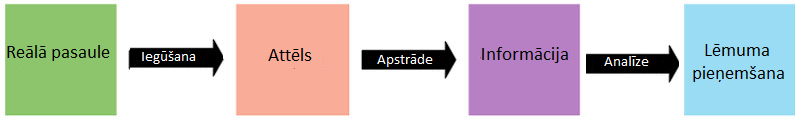
\includegraphics[height=2cm]{images/computervision1.png} %
	\caption{Datorredzes pamatprincips}%
	\label{fig:example}%
\end{figure}

Attēlu iegūšana ir process kurā reālās pasaules notikumi tiek pārveidoti bināros datos, kurus interpretē kā digitālus attēlus vai kā daļu no video fragmenta. 

Attēlu apstrāde ir iegūto attēlu zema līmeņa apstrāde. Pirmajā solī iegūtajiem binārajiem datiem pielieto algoritmus, kas norāda uz attēla daļām, kas satur zema līmeņa informāciju. Šādu informāciju var izšķirt pēc jebkādiem ģeometriskiem elementiem, kas sastāda attēlu, piemēram, punkti attēlā, attēla malas vai segmenti. Zema līmeņa attēlu apstrādes algoritmi ir malu detektēšana, segmentācijas algoritmi, klasifikācija, īpašību detektēšana.
\begin{figure}[h]%
	\centering
	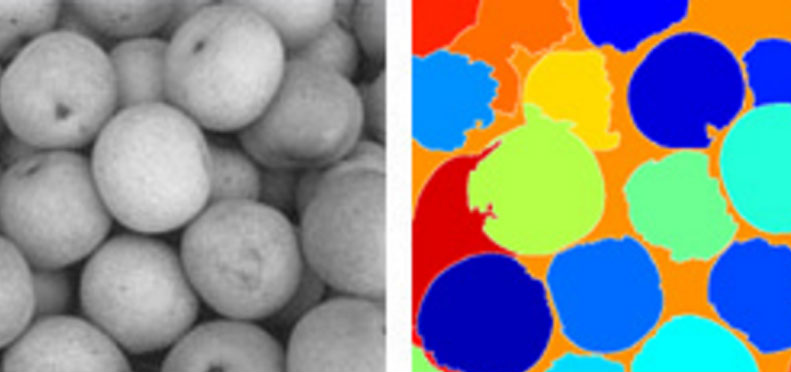
\includegraphics[height=3cm]{images/computervision2.png} %
	\caption{Ābolu segmentācija attēlā \cite{compv1}}%
	\label{fig:example}%
\end{figure} 

Pēdējā datorredzes sistēmu komponente ir attēlu analīzes solis, kurā notiks attēla analīze un pēc šī soļa datorredzes sistēmai būs iespējams pieņemt lēmumu un izvadē to atgriezt. Attēlu analīzes solī tiek pielietoti augsta līmeņa algoritmi, ņemot vērā gan attēla apstrādes solī iegūto zema līmeņa informāciju, gan pašu attēlu. Piemēri kur var izmantot šādu augsta līmeņa attēlu analīzi ir trīsdimensiju ainu atveidošana, objektu atpazīšana, objektu sekošana, cilvēku plūsmas analīze.
\begin{figure}[h]%
	\centering
	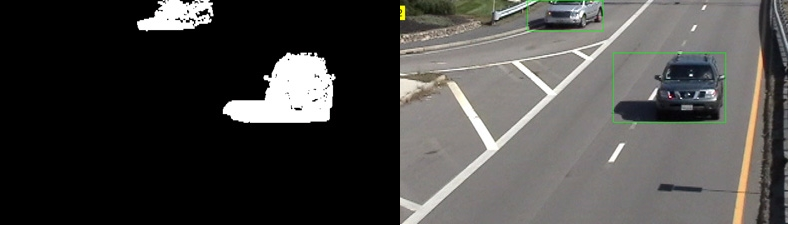
\includegraphics[height=4cm]{images/computervision3.png} %
	\caption{Objektu detektēšana pēc segmentācijas pielietošanas \cite{compv2}}%
	\label{fig:example}%
\end{figure} 

Izstrādājot datorredzes sistēmas, pētnieki saskaras ar dažādām problēmām un izaicinājumiem. Parasti šīs problēmas ir atkarīgas no datu kvalitātes, sistēmas pielietojuma un apkārtējās pasaules ietekmes uz datiem un aparatūru. Datorredzes pētnieki izstrādā risinājumus, lai padarītu datorredzes algoritmus stabilākus un efektīvākus sarežģītos uzstādījumos: nekvalitatīvi vai trokšņaini dati, reālā laika apstrāde un ierobežota skaitļošanas jauda. Mūsdienās, lai risinātu šīs problēmas, tiek savienoti mašīnmācīšanās risinājumi ar datorredzes risinājumiem.

Klasiskie datorredzes algoritmi ir smalki pētīti un optimizēti, lai iegūtu labāko veiktspēju un lai tie efektīvi izmantotu datora skaitļošanas resursus, kamēr mašīnmācīšanās algoritmi piedāvā precīzākus un vispusīgākus risinājumus, taču prasa lielus skaitļošanas resursus. Ņemot vērā iepriekš minēto, mūsdienu pētījumos ir populāri risinājumi, kas apvieno standarta datorredzes algoritmus un mašīnmācīšanās risinājumus. Labs piemērs abu šo nozaru apvienošanā ir kustīgu objektu meklēšana video fragmentos. Lai iegūtu augstāku precizitāti un taupītu skaitļošanas resursus ir iespējams attēla apstrādi veikt ar datorredzes algoritmiem un attēla analīzi (klasifikāciju, lokalizāciju, sekošanu) veikt ar neironu tīkliem.




\chapter{Literatūras apskats}
Ir aprakstītas vairākas metodes, lai veiktu cilvēku plūsmu analīzi attēlos un video fragmentos \cite{brostow2006unsupervised,chen2013cumulative,ge2009marked,chen2015person,lempitsky2010learning}. Vispārīgi, pirmie pētījumi tika vērsti uz detektēšanas veida izvēli un vai problēmu var risināt izmantojot segmentācijas metodes \cite{tu2008unified}. Šīs metodes nelabvēlīgi ietekmēja objektu nostāšanās vienam aiz otra, objektu pazušana un nekārtīgs (pārblīvēts TODO pārbaudīt tulkojumu (high clutter background)) fons attēlos. Jaunākos risinājumus var vispārīgi sadalīt trīs kategorijās: risinājumi, kas balstīti uz regresiju, risinājumi, kas balstīti uz pūļa blīvuma novērtējumu un risinājumi, kas balstīti uz konvolūcijas neironu tīkliem. 

\subsubsection{Risinājumi, kas balstīti uz regresiju}
Lai novērstu objektu paslēpšanos attēlā un pārblīvēta fona problēmas, pētnieki mēģināja skaitīt cilvēkus izmantojot regresiju. Parasti, regresija šādos risinājumos tiek veikta starp dažādām attēla īpašībām un objektu skaitu. Šāds risinājums sadala attēlu vairākos mazākos attēlos un katram šim mazajam attēlam tiek veikta aptuvenā skaita noteikšana izmantojot segmentācijas metodes. Lai noteiktu kopējo cilvēku skaitu attēlā, ir jāsaskaita katra mazā attēla aptuvenie novērtējumi. Lai apmācītu šādu sistēmu, pirmais no attēla apstrādes posmiem ir atmest attēla fonu un veikt \textit{ground-truth} novērtējumu, kas nozīmē, ka tiek manuāli izskaitīts cilvēku skaits katrā sadalītajā attēlā  \cite{chan2009bayesian,ryan2009crowd,chen2012feature}.

Šāda pieeja tika izveidota, pieņemot, ka dotajai cilvēku skaitīšanas sistēmai būtu vieglāk novērtēt cilvēku daudzumu katrā grupā atsevišķi, nevis novērtēt cilvēku daudzumu visam pūlim vienlaikus. Pieņemot, ka attēlā ir pūlis ar 20 cilvēkiem, šo pūli var sadalīt divās lielās grupās vai arī desmit pāros. Ņemot šādu attēlu vispārīgi, šāds pūļa sadalījums var nebūt tik skaidri novērtējams, jo attēlam vispārīgi būtu daudz vairāk atšķirīgu īpašību. Eksistējošas metodes, kas izmanto visu attēlu no attēla iegūst daudz vairāk īpašību, kas nozīmē, ka ir nepieciešami vairāk apmācības datu \cite{chan2008privacy}. Pētot citus rakstus var secināt, ka regresijas metodes parasti sastāv no divām lielām komponentēm: zema līmeņa īpašību iegūšanas un regresijas modeļa implementēšanas \cite{xiong2017spatiotemporal}. 

\subsubsection{Risinājumi, kas balstīti uz pūļa blīvuma novērtējumu}
Lai gan pūļu skaitīšanas risinājumi, kas balstīti uz regresiju veiksmīgi tika galā ar objektu pārklāšanās un pārblīvētā fona problēmām, tika palaista garām svarīga telpiska informācija, jo regresija tika izmantota uz lokālajām īpašībām (katra sadalītā attēla īpašībām atsevišķi). Pētījumā \cite{lempitsky2010learning} tiek piedāvāts jauns veids kā iemācīties lineāras attiecības starp sadalīto attēlu īpašībām un attiecīgās objektu blīvuma kartes izmantojot regresiju. Novērojot, ka iemācīties lineāras attiecības ir sarežģīts uzdevums, tika izveidots risinājums, kas piedāvā iemācīties nelineāras attiecības starp sadalīto attēlu īpašībām un objektu blīvuma kartēm izmantojot nejaušo mežu ietvaru (no angļu val. \textit{random forest framework}) \cite{pham2015count}. Vairāki mūsdienu risinājumi piedāvā metodes, kas balstās uz blīvuma karšu regresiju \cite{wang2016fast,xia2016block}. 

\subsubsection{Risinājumi, kas balstīti uz konvolūcijas neironu tīkliem}
Tā kā mūsdienās klasifikācijā un atpazīšanas uzdevumu risināšanā ļoti veiksmīgi darbojas uz konvolūcijas neironu tīkliem balstītas metodes. Pētnieki ir izveidojuši CNN, ar mērķi veikt pūļa skaitīšanu un blīvuma novērtējumu \cite{wang2015deep,shang2016end,walach2016learning}. Pretēji jau eksistējošajām metodēm, kas pūļa skaitu novērtē izmantojot attēla sadalīšanas metodes, Šangs \cite{shang2016end} piedāvā metodi, kas veic novērtējumu izmantojot CNN. Šī metode novērtējumu veic paralēli skaitot cilvēkus gan globālajā kontekstā, gan lokālajā kontekstā. Žangs \cite{zhang2016single} piedāvāja daudz-kolonnu arhitektūru, kas izgūst īpašības dažādos mērogos. Līdzīgi šai metodei, tika izveidots skaitīšanas modelis, kas veica novērtējumu pūļa blīvuma kartēm, ko nosauca par \textit{Hydra CNN} \cite{onoro2016towards}. Pētnieks Mardsens \cite{marsden2017resnetcrowd} pētīja pilnīgos konvolūciju neironu tīklus un vairākuzdevumu (no ang. val. \textit{multi-task}) apmācību, kuru apvienojot veica cilvēku skaitīšanu. Minētie vairākuzdevumu apmācības un daudz-kolonnu risinājumi ir sasnieguši labus rezultātus, uzrādot salīdzinoši zemu skaitīšanas kļūdu. Balstoties uz minētajiem risinājumiem var izdarīt sekojošus secinājumus \cite{sindagi2017generating}:
\begin{itemize}
	\item Šīs metodes neietver kontekstuālu informāciju, kas ir svarīgi, lai iegūtu labākus rezultātus;
	\item Lai gan eksistējošie risinājumi izmanto regresiju ar pūļa blīvuma kartēm, šie risinājumi ir vairāk balstīti uz skaitīšanas kļūdas samazināšanu, nevis blīvuma karšu kvalitātes uzlabošanu;
\end{itemize}
\newpage
Šī darba ietvaros tiks veikta skaitīšana pēc detektēšanas. Tas nozīmē, ka tiks izmantots atsevišķs objektu detektēšanas risinājums, kas objektus lokalizēs pēc konvolūciju neironu tīkla klasifikācijas atrastās klases. Kad lokalizētas visas objekta instances, skaitīšanas uzdevums paliek elementārs. Taču objektu detektēšanas problēmām nav atrasti risinājumi, kas strādā nevainojami, it īpaši, ja vairākas objektu instances attēlā pārklājas. Vienkāršākie objektu detektēšanas risinājumi balstās uz divām operācijām: izveidot reālu vērtību pārliecības (no angļu val. \textit{confidence}) karti un izmantojot šo karti, tiek meklētas augstās vērtības, kas atbilst individuālām objektu instancēm. Vairākas metodes pieņem, ka attēlos ir vairāki vienādi objekti un tos vienu no otra var atšķirt izmantojot \textit{Monte-Carlo} procesu \cite{descombes2009object}, morfoloģisko analīzi \cite{selinummi2005software} un variāciju optimizāciju \cite{nath2006cell}. Mūsdienās, populārākās un precīzākās metodes objektu detektēšanai ir \textit{YOLO} (\textit{You Only Look Once}) \cite{redmon2016you}, \textit{Faster-RCNN} (\textit{Faster Region-Based Convolutional Neural Network}) \cite{ren2015faster} un \textit{SSD} (\textit{Single Shot MultiBox Detector}) \cite{liu2016ssd}.
\subsubsection{YOLO (\textit{You Only Look Once})}
\textit{YOLO} pārveido objektu detektēšanas problēmu par vienkāršas regresijas problēmu, veicot regresiju starp attēla pikseļiem, ierobežojošo logu (no angļu val. \textit{bounding box}) koordinātēm un klašu varbūtībām. Viens konvolūciju neironu tīkls vienlaicīgi veic daudz ierobežojošo logu prognozes un klašu varbūtības šiem logiem. Šādam modelim ir vairākas priekšrocības salīdzinājumā ar citām objektu detektēšanas metodēm: 
\begin{itemize}
	\item Tas ir ļoti ātrs. Tā kā detektēšana tiek pārvērsta par parastu regresijas problēmu, nav nepieciešams sarežģīts vairāku procesu kopums. 
	\item Kad \textit{YOLO} izdara prognozes par attēlu, tiek ņemts viss attēls kopumā. Pretēji slīdošo logu metodēm un uz reģionu minējumiem balstītajām metodēm, \textit{YOLO} sistēma apmācības laikā redz visu attēlu, tādējādi tas ir spējīgs netieši klasēm pievienot to kontekstuālo informāciju.
	\item \textit{YOLO} iemācās vispārējus objektu attēlojumus, kas nozīmē, ka pielietojot šo sistēmu tam nepazīstamiem datiem vai negaidītiem ievades datiem, ir salīdzinoši mazāka iespēja, ka tas kļūdīsies. 
\end{itemize}

\textit{YOLO} detektēšanas sistēma sadala ievades attēlu režģī. Ja objekta centrs trāpās kādā no režģa šūnām, tad šī šūna ir atbildīga par šī objekta detektēšanu. Katra šūna prognozē noteiktu ierobežojošo logu (\textit{bounding boxes}) skaitu, kā arī pārliecības rezultātus (\textit{confidence scores}) šiem logiem. Šie pārliecības rezultāti norāda cik pārliecināta ir sistēma par to ka ierobežojošajos logos ir objekts un cik precīzi ir novietots pats ierobežojošais logs. Pārliecību matemātiski izsaka kā objekta varbūtības un \textit{IoU} (\textit{intersection over union}) reizinājumu. Ja šūnā nav neviena meklētā objekta, tad pārliecības rezultāts būs nulle.

\begin{figure}[h]%
	\centering
	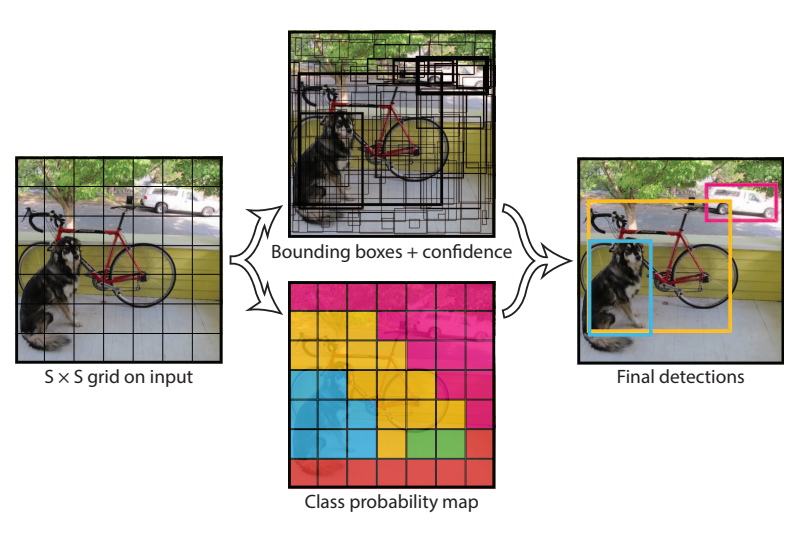
\includegraphics[height=6cm]{images/yolo.png} %
	\caption{\textit{YOLO} modelis \cite{redmon2016you}}%
	\label{fig:example}%
\end{figure}

Katrs ierobežojošais logs satur piecas prognozes: koordinātes, kas norāda loga centru attiecībā pret režģa šūnām, loga augstuma un platuma vērtības un pārliecības vērtību. Katra šūna prognozē nosacītās klašu varbūtības. Neatkarīgi no atrasto ierobežojošo logu skaita, katrai šūnai tiks piešķirta tikai viena klase.

Pētījumā \cite{redmon2016you} minētajai standarta \textit{YOLO} sistēmai ir 24 konvolūcijas slāņi, kam seko 2 pilnīgi savienotie slāņi. Pirmie konvolūcijas slāņi iegūst attēlu īpašības, kamēr pilnīgi savienotie slāņi prognozē objektu varbūtības un koordinātes.

\begin{figure}[h]%
	\centering
	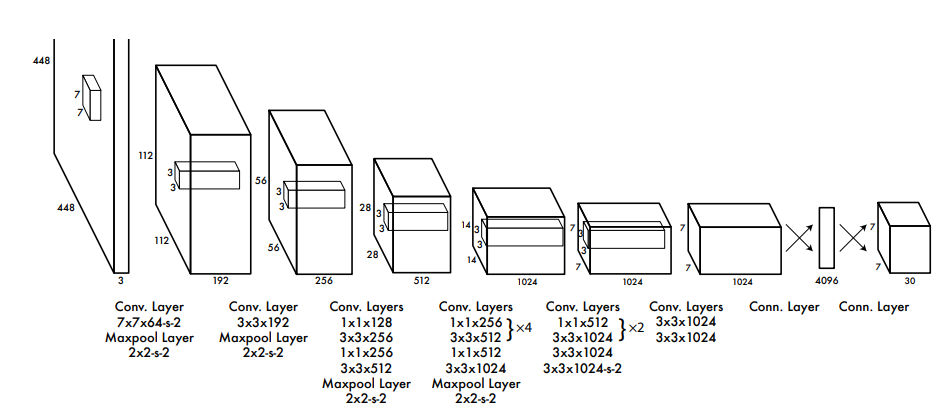
\includegraphics[height=7cm]{images/yoloarch.png} %
	\caption{\textit{YOLO} tīkla arhitektūra \cite{redmon2016you}}%
	\label{fig:example}%
\end{figure}
\newpage
Lai gan \textit{YOLO} ir labs un ātrs risinājums objektu detektēšanā, tam ir savi ierobežojumi:
\begin{itemize}
	\item Šī sistēma uzliek telpiskus limitus ierobežojošo logu prognozēm, jo katra režģa šūna prognozē tikai divus logus un katrai šūnai var piešķirt tikai vienu klasi. Šāds telpisks ierobežojums, limitē cik tuvumā esošus objektus \textit{YOLO} modelis var atrast. Tas nozīmē, ka sistēmai problēmas sagādā mazi objekti, kas atrodas grupās, piemēram, putni.
	\item Līdzīgi kā citas objektu detektēšanas metodes, \textit{YOLO} iemācās veikt ierobežojošo logu prognozes balstoties uz apmācības datiem, kas nozīmē, ja objektu detektēšana jāveic attēliem ar neierastiem izmēriem vai uzstādījumiem, \textit{YOLO} var būt grūti izšķirt objektus šajos attēlos.
	\item Attēlā 2.2 ir redzams, ka tīkla arhitektūrā ir vairāki apvienošanas slāņi (\textit{Maxpool layer}), kas nozīmē, ka ierobežojošo logu prognozēšanā tiek izmantotas salīdzinoši zemas kvalitātes (no angļu val. \textit{coarse}) īpašības. 
	\item Apmācības laikā izmantotā \textit{loss} funkcija pieņem, ka kļūdas mazajos ierobežojošajos logos ir tik pat būtiskas kā kļūdas lielajos logos, kas nav labs risinājums. Mazai kļūdai lielā logā ir maza ietekme, taču tikpat mazai kļūdai mazā logā var būt liela ietekme uz pārliecības rezultātiem. 
\end{itemize}   

\subsubsection{Faster-RCNN (\textit{Faster Region-Based Convolutional Neural Network})}
\textit{Faster-RCNN} ir objektu detektēšanas sistēma, kas sastāv no diviem tīkliem: reģionu noteikšanas tīkla (no angļu val. \textit{region proposal network}) jeb RPN, kas veido reģionu priekšlikumus, un no tīkla, kas šiem reģioniem veic objektu detektēšanu. RPN atgriež vairākus logus jeb priekšlikumus, kurus novērtēs klasifikators un regresors, lai noteiktu objektu esamību konkrētajā logā.

\begin{figure}[h]%
	\centering
	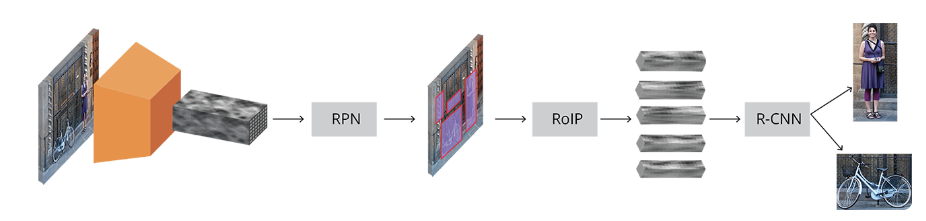
\includegraphics[height=3.5cm]{images/fastercnnarch.png} %
	\caption{\textit{Faster R-CNN} arhitektūra \cite{fasterrcnn}}%
	\label{fig:example}%
\end{figure}
\textit{Faster R-CNN} sistēmai ir salīdzinoši sarežģīta arhitektūra. Neiedziļinoties sīkumos, šī modeļa arhitektūra (attēls 2.3) sākas ar attēlu no kura ir nepieciešams iegūt: sarakstu ar ierobežojošajiem logiem, katram loga marķējumu (klases nosaukums) un katra marķējuma un ierobežojošā loga varbūtību. 

Ievades attēls ir vairākdimensiju masīvs, kuru padod ievadē konvolūcijas neironu tīklam līdz tiek iegūta īpašību karte. Pēc īpašību kartes iegūšanas, tā tiek nodota RPN. Izmantojot šīs īpašības, tīkls meklē iepriekš definētu skaitu ar reģioniem (ierobežojošajiem logiem, kurus sauc par \textit{anchors}), kuri var saturēt objektus (RPN nav svarīgi noskaidrot kādas klases objekts atrasts, tikai vai reģionā ir kāds objekts vai reģions satur tikai fona informāciju).  Šie reģionu logi ir fiksēta izmēra ierobežojošie logi, kuri ir vienmērīgi izvietoti attēla robežās. Pēc tam kad iegūts saraksts ar iespējamiem objektiem un to atrašanās vietām attēlā, detektēšanas problēma paliek krietni vienkāršāka. Izmantojot no konvolūcijas neironu tīkla iegūtās īpašību kartes un reģionu logus ar atbilstošajiem objektiem, pielieto RoI (no angļu val. Region of Interest) apvienošanu.
\begin{figure}[h]%
	\centering
	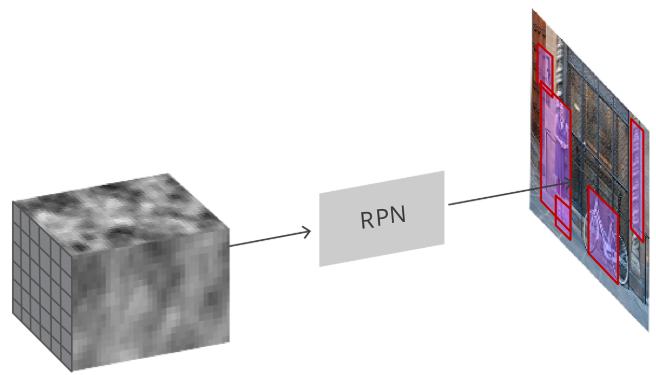
\includegraphics[height=5cm]{images/rpnstep.png} %
	\caption{RPN arhitektūra. RPN ievadē saņem no CNN atgriezto īpašību karti un attēlā ģenerē reģionu priekšlikumus. \cite{rpnarch}}%
	\label{fig:example}%
\end{figure}
Pēc RPN soļa ir iegūti vairāki prognozētie objekti, taču nav zināms kāda ir šo objektu klase. Vienkāršākais veids kā katram reģionam atrast klasi ir, samazināt šo reģionu un padot apmācītam tīklam, kas izmantojot iepriekš iegūtās attēla īpašības varēs risināt klasifikācijas problēmu, taču šāds risinājums nav efektīvs. Lai veiktu šāda veida klasifikāciju 1000 priekšlikumiem, tiks patērēts daudz laika un skaitļošanas resursu. Šo problēmu, \textit{Faster R-CNN} izstrādātāji risina vai vismaz samazina, izmantojot RoI apvienošanu \cite{roipooling}, ņemot iepriekš iegūto īpašību karti un iegūtos reģionus. 

Pēc RoI apvienošanas soļa seko R-CNN daļa, kas klasificē reģionu logu saturu vai arī atmet to, norādot reģiona marķējumā, ka tas ir fons. Kā arī R-CNN tīkls atjauno reģionu ierobežojošo logu koordinātes, lai ierobežojošais logs precīzāk pārklātu objektu. R-CNN izmanto katra piedāvātā reģiona īpašību karti, saplacina (no angļu val. \textit{flattens}) to un izmanto divus pilnīgās savienošanas slāņus ar ReLU kā aktivizācijas funkciju un atgriež objekta varbūtību un atjaunotā ierobežojošā loga robežas.

\begin{figure}[h]%
	\centering
	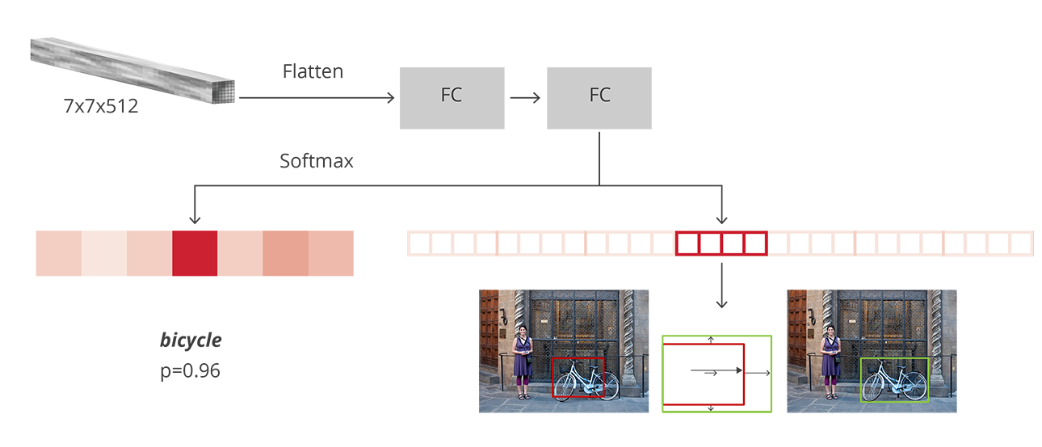
\includegraphics[height=5cm]{images/rcnnarch.png} %
	\caption{R-CNN arhitektūra \cite{fasterrcnn}}%
	\label{fig:example}%
\end{figure}

Līdzīgi kā pēc RPN soļa, pēc R-CNN soļa ir iegūti objekti, kuriem ir atrastas klases un kurus ir nepieciešams papildus apstrādāt. Lai  katram reģionam pielietotu ierobežojošo logu labojumus, tiek ņemts vērā kuras klases atrastā varbūtība bija ar visaugstāko vērtību (ja reģiona augstākā varbūtība ir klase "fons", tad šis reģions tiek ignorēts). Pēc gala objektu iegūšanas un "fona" objektu atmešanas, tiek pielietots uz klasēm balstīts NMS (\textit{non-maximum suppression}), lai novērstu vienas un tās pašas objekta instances detektēšanu vairākos reģionos \cite{hosang2017learning}.

\subsubsection{SSD (\textit{Single Shot MultiBox Detector})}

Īsumā, \textit{SSD} galvenā ideja ir tāda, ka tiek izmantots tikai viens neironu tīkls, kas padara risinājumu ātru un nav nepieciešamība pēc reģionu priekšlikumiem. Tā vietā, tiek izmantotas dažādi ierobežojošie logi, kuri tiek mainīti prognožu izdarīšanas laikā. Pētījums par \textit{SSD} kļuva pieejams 2016. gadā \cite{liu2016ssd} un šī detektēšanas sistēma uzstādīja jaunus rekordus veiktspējā un precizitātē objektu detektēšanas uzdevumu veikšanai. Lai labāk saprastu \textit{SSD} ir vērtīgi izskaidrot šīs sistēmas pilno nosaukumu:
\begin{itemize}
	\item \textit{\textbf{Single Shot}} : tas nozīmē, ka objektu lokalizācijas un klasifikācijas uzdevumus tiek veikts neironu tīkla slāņiem izejot cauri vienu reizi;
	\item \textit{\textbf{MultiBox}} : ir ierobežojošo logu regresijas tehnika, kuru izveidoja pētnieki, kas strādāja ar pie \textit{SSD} izveides;
	\item  \textit{\textbf{Detector}} : \textit{SSD} sistēmā neironu tīkls ir objektu detektors, kas arī klasificē detektētos objektus;
\end{itemize}
\newpage
\begin{figure}[h]%
	\centering
	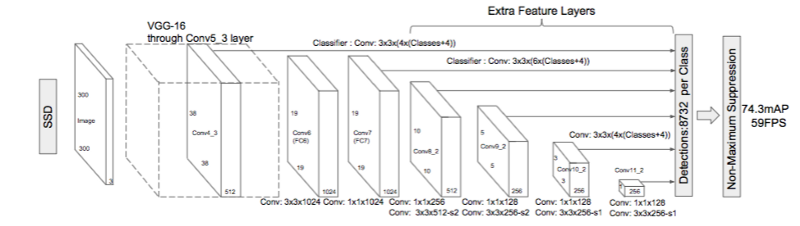
\includegraphics[height=4.5cm]{images/ssdarch.png} %
	\caption{SSD arhitektūra \cite{ssdarch}}%
	\label{fig:example}%
\end{figure}

Attēlā 2.6 ir attēlota \textit{SSD} arhitektūra, kur parādīts, ka šī objektu detektēšanas sistēma ir balstīta uz \textit{VGG Net} arhitektūru, taču netiek izmantoti standarta arhitektūras pilnīgi savienotie slāņi. \textit{VGG Net} neironu tīkla arhitektūra tiek izmantota kā \textit{SSD} bāze, jo tā darbojas ar augstu veiktspēju attēlu klasifikācijas uzdevumu veikšanā \cite{simonyan2014very}. Tai vietā, lai \textit{SSD} izmantotu pilnīgi savienotos slāņus no standarta \textit{VGG Net} konfigurācijas, tiek izmantoti papildus konvolūcijas slāņi, lai būtu iespējams iegūt attēla īpašības dažādos attēla izmēros un samazinātu katra nākamā slāņa ievadē saņemto attēlu izmēru. 

\textit{MultiBox} ir ierobežojošo logu regresijas metode, kas balstīta uz \textit{SSD} izstrādātāju pētījumu par objektu ierobežojošo logu koordināšu priekšlikumiem \cite{szegedy2014scalable}, kur nav zināmas objektu klases. \textit{MultiBox} \textit{loss} funkcija apvieno divas objektu detektēšanas mērvienības: \textit{confidence loss} un \textit{location loss}. \textit{Confidence loss} mēra, cik pārliecināts ir tīkls, ka aprēķinātais ierobežojošais logs satur objektu. \textit{Location loss} mēra cik tālu no tīkla prognozētajiem ierobežojošajiem logiem atrodas \textit{ground-truth} ierobežojošie logi apmācības datos. \textit{MultiBox loss} aprēķina sekojoši:

\begin{equation*}
\var{multibox_loss}
= \var{confidence_loss}
+ \var{alpha}
* \var{location_loss}
\end{equation*}
\textit{Alpha} minētajā vienādojumā palīdz balansēt \textit{location loss} vērtību. Līdzīgi kā citām dziļās mašīnmācīšanās sistēmām, ir nepieciešams atrast vienādojuma parametrus, kas vislabāk samazina \textit{loss} funkciju, tādējādi pietuvinot tīkla prognozes \textit{ground-truth} vērtībām.

\textit{MultiBox} pētnieki veidojot šo metodi ieviesa jaunu terminu \textit{priors}. \textit{Priors} ir iepriekš aprēķināti, fiksēta izmēra ierobežojošie logi (\textit{Faster R-CNN} sistēmā šos logus sauc par \textit{anchors}), kas cieši sakrīt ar \textit{ground-truth} ierobežojošo logu izvietojumu. Balstoties uz šiem iepriekš aprēķinātajiem ierobežojošiem logiem, \textit{MultiBox} tos izmanto kā prognozes un mēģina regresēt tuvāk \textit{ground-truth} ierobežojošajiem logiem. Beigās \textit{MultiBox} saglabā tikai labākās prognozes ar minimizētām \textit{location loss} un \textit{confidence loss}. 

\textit{SSD} pētījumā ir veikti uzlabojumi standarta \textit{MultiBox} sistēmai, kas padara šo objektu detektēšanas sistēmu vēl spējīgāku lokalizēt un klasificēt objektus. \textit{SSD} katra īpašību kartes šūna ir savienota ar dažādu izmēru un dažādu proporciju ierobežojošajiem logiem (\textit{priors}). Šie logi ir manuāli izvēlēti, kas, teorētiski, ļauj \textit{SSD} darboties ar dažādi konfigurētiem ievades datiem. Pieņemot, ka ir definēts \textit{c} skaits klašu, katrai īpašību kartes šūnai ir definēts \textit{b} skaits ierobežojošo logu un īpašību kartes izmērs ir \textit{f}, \textit{SSD} aprēķinātu \textit{f * b * (4 + c)}
vērtības šai īpašību kartei. 

\begin{figure}[!htb]
	\minipage{0.32\textwidth}
	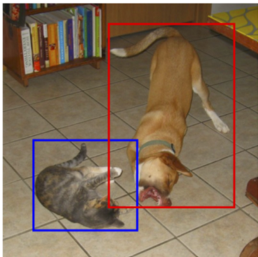
\includegraphics[width=\linewidth]{images/ssdgtboxes.png}
	\caption{Attēls ar \textit{ground-truth} logiem \cite{liu2016ssd}}
	\endminipage\hfill
	\minipage{0.32\textwidth}
	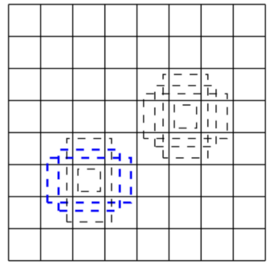
\includegraphics[width=\linewidth]{images/ssd88featmap.png}
	\caption{8 x 8 izmēra īpašību karte \cite{liu2016ssd}}
	\endminipage\hfill
	\minipage{0.32\textwidth}%
	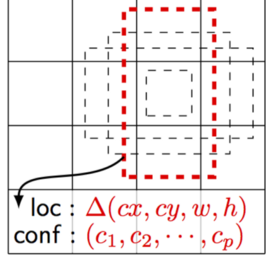
\includegraphics[width=\linewidth]{images/ssd44featmap.png}
	\caption{4 x 4 izmēra īpašību karte \cite{liu2016ssd}}
	\endminipage
\end{figure}

Attēlā 2.7 ir parādīts, ka apmācības laikā \textit{SSD} ir tikai nepieciešams ievades attēls un \textit{ground-truth} logi, kas atspoguļo objektus attēlā. Izmantojot konvolūcijas principus, tiek novērtēti daži ierobežojošie logi, dažādos attēla mērogos un tie tiek uzglabāti īpašību kartēs ar dažādiem izmēriem (attēlā 2.8 ir parādīta 8x8 izmēra īpašību karte un attēlā 2.9 4x4 izmēra īpašību karte). Katram logam aprēķina formas nobīdi no patiesās un pārliecības vērtības katrai objektu kategorijai (attēlā 2.9 c1,c2,...,cp). Apmācības laikā, definētie logi tiek pieskaņoti \textit{ground-truth} logiem. Piemēram, attēlā 2.7 parādīts, ka divi ierobežojošie logi ir pieskaņoti kaķim un sunim. Modeļa \textit{loss} (modeļa kopējā precizitāte ņemot vērā apmācības un validācijas datus) ir svērtā summa starp \textit{localization loss} un \textit{confidence loss}. 

Līdzīgi \textit{Faster-RCNN}, arī \textit{SSD} kā vienu no pēdējiem soļiem tīkla izpildes laikā izmanto \textit{non-maximum suppression} (NMS). Pēc detektēšanas soļa iegūtie logi tiek šķiroti pēc norādīta sliekšņa, kas atkarīgs no \textit{confidence loss} vērtības. Tikai labākos logus saglabā un pārējie (mazāks \textit{confidence loss} par sliekšņa vērtību) tiek atmesti. NMS pielietošana nodrošina, ka tikai labākās logu prognozes tīkls saglabās un trokšņainās atmetīs.
 \newpage
\begin{figure}[h]%
	\centering
	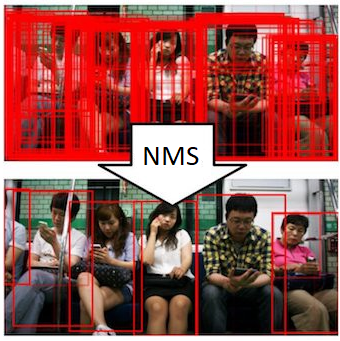
\includegraphics[height=4cm]{images/nms.png} %
	\caption{\textit{Non-maximum supression} piemērs \cite{liu2016ssd}}%
	\label{fig:example}%
\end{figure}

\textit{SSD} pētījumā \cite{liu2016ssd} ir aprakstīti novērojumi par sistēmas darbību:
\begin{itemize}
	\item Jo vairāk iepriekš definētie logi, jo precīzāk notiek detektēšana, taču tas negatīvi ietekmē sistēmas ātrumu;
	\item Izmantojot \textit{MultiBox} vairākos slāņos, sistēma objektu detektēšanu veic precīzāk, jo detektors tad darbojas ar dažādu izšķirtspēju īpašībām;
	\item \textit{SSD} mēdz jaukt objektus, kam ir līdzīgas klases (piemēram, dzīvnieki ar 4 kājām);
	\item \textit{SSD} vāji strādā ar maziem objektiem, jo tie var neuzrādīties visās īpašību kartēs. Palielinot ievades attēlu izšķirtspēju ir iespējams samazināt šo problēmu.
\end{itemize}

Ņemot vērā tikai pētījumos \cite{redmon2016you,ren2015faster,liu2016ssd} pieejamo informāciju, dotajā brīdī, \textit{Faster R-CNN} ir labākā objektu detektēšanas sistēma, ja vērā ņem tikai precizitātes vērtējumus un lietotājam ir pieejami neierobežoti skaitļošanas resursi. Ja lietotājiem ir ierobežoti skaitļošanas resursi, \textit{SSD} ir labākais ātruma un precizitātes kompromiss. Ja par precizitāti nav jāuztraucas, bet ir vēlme pēc ļoti ātras sistēmas, tad labākais variants ir \textit{YOLO}. Lai gan \textit{Faster R-CNN} labāk par pārējiem spēj atrast maza izmēra objektus, sistēma ir lēna un nenodrošina reālā laika detektēšanu. Gan \textit{YOLO}, gan \textit{SSD} sistēmas nodrošina reālā laika objektu detektēšanu, kas ir nepieciešams šī darba ietvaros. Ņemot vērā augstāk minēto informāciju, pētījuma ietvaros radītais risinājums izmantos \textit{SSD} objektu detektēšanas sistēmu, jo tā ir labākā precizitātes un ātruma apvienojums un apmācību ir iespējams veikt ar lietotājiem pieejamākām ierīcēm. 

Pēc objektu detektēšanas metodes izvēlēšanās, šī pētījuma ietvaros ir nepieciešams apskatīt sekošanas risinājumus, kuru izmantot gala risinājumā. Lai veiksmīgi veiktu cilvēku plūsmas analīzi, ar izvēlēto objektu detektēšanas metodi vien nepietiek, objektiem ir arī jāseko. Šādā risinājumā ir vērtīgi ieviest sekošanas risinājumu sekojošu iemeslu dēļ:
\begin{itemize}
	\item Sekošanas algoritmi darbojas ātrāk kā detektēšanas algoritmi. Šādu argumentu var izskaidrot ar to, ka sekojot objektam, kas jau ir atrasts iepriekšējā kadrā, sistēmai ir pieejama informācija par objekta attēlojumu, atrašanās vietu, kustības virzienu un kustības ātrumu. Sekošanas algoritms izmantos visu šo informāciju, lai nepazaudētu objekta atrašanās vietu, kamēr objektu detektēšanas algoritmam katrs katrs ir jāapstrādā no jauna.
	\item Sekošanas algoritmi ir kā drošības tīkls gadījumā, ja detektēšanas risinājumi vairs nevar atrast kādu no iepriekšējos kadros noteiktajiem objektiem. Piemēram, ja starp objektu un video kameru nostājas šķērslis, tas detektēšanas risinājumiem sagādās pamatīgas problēmas, kamēr labs sekošanas risinājums nepazaudētu objekta atrašanās vietu.
	\item Sekošanas algoritmi veido savienojumus starp video kadriem, tādā veidā saglabājot objekta identitāti.
\end{itemize}

Sekošanas mērķis ir atrast objektu dotajā video kadrā, pieņemot, ka objektam ir veiksmīgi sekots visos iepriekšējos kadros vai dotajā kadrā pirmo reizi atrasta šī objekta instance. Tā kā objektam ir sekots līdz dotajam kadram, ir zināms, ka objekts kustas, kas nozīmē, ka ir zināmi kustības modeļa parametri. Kustības modeli veido iepriekšējos kadros noteiktā objekta atrašanās vieta un ātrums. Nezinot neko citu kā kustības modeļa parametrus jau ir iespējams izteikt diezgan precīzu minējumu kur dotajā kadrā varētu atrasties objekts. Risinot sekošanas problēmu video fragmentos, ir pieejama informācija par vairāk kā tikai objekta kustību ir zināms arī objekta izskats visos iepriekšējos kadros. Zinot objekta izskatu, ir iespējams veidot izskata modeli, šādu modeli var izmantot, lai precizētu objekta atrašanās vietu pēc tam, kad balstoties uz kustības modeli ir izdarīts minējums par aptuveno objekta atrašanās vietu. Ja objekts ir vienkāršs un starp kadriem izskatu nav mainījis, tad izskata modeli var izmantot kā veidni, kuru meklēt jaunajā kadrā. Diemžēl, objekta izskats var pamatīgi mainīties, lai cīnītos ar šo problēmu modernie sekošanas risinājumi izmanto izskata modeli kā klasifikatoru, kurš tiek apmācīts algoritma izpildes laikā. 

Gala risinājuma izstrādes laikā tika apskatīti \textit{OpenCV} programmatūrā piedāvātie sekošanas algoritmi: \textit{Multiple Instance Learning} (MIL) un \textit{AdaBoost} kā arī \textit{SiamFC} sekošanas algoritms, kas neietilpst \textit{OpenCV} bibliotēkā, bet ir aprakstīts Luka Bertinetto pētījumā \cite{bertinetto2016fully}.

\subsubsection{Multiple Instance Learning}

\subsubsection{AdaBoost}
\subsubsection{SiamFC}
\chapter{Plūsmas analīzes algoritma implementācija}
Plūsmas analīzes algoritma implementācija tika veidota programmēšanas valodā \textit{Python}, izmantojot \textit{caffe}. Šis ietvars tika izmantots, lai veiktu \textit{VGG Net} konvolūcijas neironu tīkla modelēšanu un apmācību objektu klasificēšanai un implementētu \textit{SSD} algoritmu objektu detektēšanai. Lai gan gala risinājums tika veidots izmantojot \textit{SSD} algoritmu, lai rastu plašāku ieskatu pieejamajos risinājumus, tika apskatīts arī \textit{YOLO} objektu detektēšanas algoritms, kas implementēts \textit{darknet} ietvarā.

Neatkarīgi no objektu detektēšanas algoritma un ietvara, kurā tas implementēts, gala risinājums sastāv no četrām daļām: datu kopas sagatavošanas, konvolūcijas neironu tīkla apmācības, objektu detektēšanas algoritma implementācijas un sekošanas algoritma implementācijas. Pēc datu sagatavošanas, tiek veikta konvolūcijas neironu tīkla apmācība,  lai tas būtu spējīgs klasificēt attēlos vai video fragmentos esošos objektus. Kad apmācīts pietiekami precīzs modelis, to katrā kadrā izmanto objektu detektēšanas algoritms, lai meklētu objektus. Kad objekts atrasts, tā vietā tiek inicializēts sekošanas algoritms, kas nākamajos kadros noteiks objekta atrašanās vietu, ja to vairs nebūs iespējams detektēt. 
\section{Cilvēku galvas noteikšanas datu sagatavošana}
Lai veiksmīgi apmācītu konvolūcijas neironu tīklus objektu detektēšanai, ir nepieciešama liela datu kopa ar meklējamo objektu piemēriem, šajā gadījumā ar cilvēku galvu attēliem. Jo vairāk datu, jo dažādākus objektus apmācītais tīkls spēs klasificēt. Šī darba nolūkos interesējošie piemēri ir cilvēku galvu attēli un ir pieejamas vairākas datu kopas, autors šī darba nolūkos ir izvēlējies \textit{HollywoodHeads} datu kopu \cite{vu15heads}. 

\textit{HollywoodHeads} datu kopa satur 369 846 cilvēku galvu anotācijas (anotācija ir \textit{XML} formāta fails, kas piekārtots katram datu kopas attēlam un satur informāciju par attēlu, par objektu, kādi objekti redzami attēlā un šo objektu ierobežojošie logi), 224 740 video kadros no 21 Holivudas filmām\footnote{Filmu saraksts: American beauty, As Good As It Gets, Big Fish, Big Lebowski, Bringing out the
dead, Capote, Clerks, Crash, Dead Poets Society, Double Indemnity, Erin
Brockovich, Fantastic 4, Fargo, Fear And Loathing In Las Vegas, Fight	Club,Five Easy Pieces, Forrest Gump, Gang Related, Gandhi, Charade, I Am Sam}. Šīs filmas ir no dažādiem žanriem un laika brīžiem vēsturē, lai piedāvātu visdažādākos galvu piemērus. Lai izveidotu anotācijas, datu kopas veidotāji manuāli atlasīja cilvēku galvas no rīcības bagātām ainām. Katrai galvai manuāli tika izveidoti ierobežojošie logi (mazākais iespējamais laukums, kurā ietilpst visi galvas redzamie pikseļi), vairāku kadru garumā. Kopā tika savākti dati no 2 380 klipiem ar 3 872 apsekotiem cilvēkiem, kas kopā veido vairāk kā 3.5 stundas ar video fragmentiem. Datu kopa ir sadalīta apmācības, validācijas un testēšanas apakškopās un šīs apakškopas, filmu ziņā, nepārklājas. \textit{HollywoodHeads} apmācības datu apakškopa satur 216 719 kadrus no 15 filmām, validācijas apakškopa satur 6 719 kadrus no 3 filmām un testēšanas apakškopa satur 1 302 kadrus no 3 filmām. Cilvēku galvas, kurām priekšā ir šķēršļi vai ir slikts apgaismojums ir anotācijās apzīmētas kā "sarežģīti" (no angļu val. \textit{difficult}) piemēri un netiek izmantoti apmācības laikā. 

Diemžēl, izvēlēto datu kopu gan nav iespējams uzreiz pielietot apmācībā, jo formāts kādā strukturēti dati vienmēr nav saderīgs ar formātu kādu sagaida ietvars, šajā gadījumā \textit{caffe} un \textit{darknet}. Konvolūciju neironu tīklu apmācībā populāras datu kopas ir: \textit{COCO} \cite{lin2014microsoft}, \textit{PASCAL VOC} \cite{everingham2010pascal} un \textit{ILSVRC} \cite{ILSVRC15}. \textit{Caffe} un \textit{darknet} ietvaros ir iebūvēta iespēja apmācīt CNN ar visām minētajām datu kopām, izņemot \textit{HollywoodHeads} datu kopu. Šīs problēmas risinājums gan nav sarežģīts. Autors aizstāja \textit{VOC} datu kopas attēlus un anotācijas (anotāciju struktūra abām datu kopām sakrīt un specifiski anotāciju pārveidojumi nav nepieciešami) ar \textit{HollywoodHeads} datu kopas attēliem un anotācijām un gan \textit{caffe}, gan \textit{darknet} uzstādījumos bija nepieciešams nomainīt klašu skaitu. \textit{Caffe} gadījumā klašu skaits no 20 (\textit{VOC} gadījumā) tika samainīts uz 2 klasēm (galva un fons), kamēr \textit{darknet} gadījumā klašu skaits no 20 tika samainīts uz 1 klasi (galva).

Nākamais solis datu sagatavošanā \textit{caffe} ietvaram ir izveidot \textit{LMDB} (\textit{Lightning Memory-Mapped Database}), kurā iekodēs attēlu informāciju. \textit{LMDB} ir ļoti augstas veiktspējas, kompakta datu glabātuve, kas izmanto atmiņā kartētus failus, lai varētu lasīt datus ar augstu veiktspēju, tai pašā laikā saglabājot standarta uz diskiem balstīto datu glabātuvju ietilpību. Apmācības, validācijas un testēšanas datu apakškopām katrai būs sava \textit{LMDB} datu glabātuve ar saitēm uz pašu datu kopu. \textit{Bash} skripts, kas izveidos šīs datubāzes ir ievietots pielikumā \ref{appendix:pielikums1}. Papildus datubāzēm, lai sāktu apmācību ir nepieciešams ģenerēt teksta failus, kuros norādītas apmācības, validācijas un testēšanas attēlu atrašanās vietas datorā.

\textit{Darknet} ietvara gadījumā, no \textit{VOC} formāta datiem ir nepieciešams izveidot marķējumu (no angļu val. \textit{label}) failus, kas no anotāciju failiem iegūs attēlos esošo objektu ierobežojošo logu izmērus un atrašanās vietas un klasi kurām pieder šie logi. Marķējumu faili katrā rindā satur informāciju par vienu no ierobežojošajiem logiem, formātā :\\ $<objekta-klase> <x> <y> <platums> <augstums>$.\\
Kur \textit{x,y, platums, augstums} ir atkarīgi no attēla platuma un augstuma. Lai automātiski izveidotu marķējumu failus katram attēlam, ir nepieciešams palaist \textit{Python} programmēšanas valodā rakstītu skriptu, kas pievienots pielikumā \ref{appendix:pielikums2}. Šis skripts nolasa katru anotācijas failu un atkarībā no anotācijas failā atrastajiem parametriem, katram attēlam izveido marķējumu failu ar iepriekš minēto informāciju un izveido teksta failus, kuros norādītas apmācības, validācijas un testēšanas attēlu atrašanās vietas datorā. Kad šie datu glabātuvju un datu sadalījumu faili ir ģenerēti, ir iespējams sākt tīkla apmācību.
\section{Konvolūcijas neironu tīkla apmācība}
Lai veiksmīgi apmācītu konvolūciju neironu tīklus, ir nepieciešama ierīce ar jaudīgu \textit{GPU} jeb \textit{Graphics Processing Unit}. \textit{GPU} kalpo, lai skaitļošanas jaudu izdalītu datora jeb citu ierīču grafiskajiem procesoriem, kuri sastāv no simtiem kodolu un katrs kodols ir spējīgs paralēli izpildīt kādu darbību. Izmantojot \textit{CPU} jeb \textit{Central Processing Unit}, lietotājiem ir pieejami kodolu skaits sākot no 1 līdz 16. Šī darba nolūkos, konvolūciju neironu tīkli tika apmācīti izmantojot \textit{NVIDIA GeForce GTX 1080} grafisko procesoru, kam pieejami 2 560 kodoli un 8 GB operatīvā atmiņa. Apmācības procesa konfigurēšana katram ietvaram atšķiras.

\paragraph{\textit{SSD} detektēšanas sistēmas apmācība izmantojot \textit{caffe} ietvaru}
\hfill\par
Pēc datu sagatavošanas ir nepieciešams izvēlēties tīkla arhitektūru ar kuru notiks apmācība. \textit{Caffe} ietvarā ir ļoti elementāri izveidot pašam savu arhitektūru, taču nav iespējams paredzēt cik precīza būs šī arhitektūra, tāpēc labāk izvēlēties kādu no \textit{caffe} jau piedāvātajām, piemēram, \textit{GoogLeNet} vai \textit{AlexNet}. Ar darbā izmantoto grafisko skaitļošanas iekārtu nav iespējams efektīvi apmācīt ļoti sarežģītus tīklus, tāpēc \textit{SSD} apmācībā tika izmantota \textit{VGG Net} arhitektūra, ar kuru apmācības laiki nebūs ļoti gari un kas ir pielāgota \textit{caffe} ietvaram \cite{ssdmodel}. Pēdējās darbības pirms sākt apmācību ir risinātāja (no angļu val. \textit{solver}) un tīkla modeļa konfigurācijas failu pielabošana (ieskaitot apmācības parametrus kā filtru skaitu, klašu skaitu, cik attēlus vienlaicīgi piedāvāt apmācībai), lai apmācībai izmantotu pirms tam sagatavotos datus ar tikai vienu klasi. Pēdējais solis pirms apmācības sākšanas ir sākuma svaru iegūšana, kas ir publiski pieejami lejupielādei. Pēc sākuma svaru lejupielādēšanas, apmācība var sākties. 

\textit{SSD} gadījumā, lai zinātu, kad pārtraukt apmācību, autors novēroja \textit{mAP} jeb \textit{Mean Average Precision} metriku un \textit{loss} funkcijas atgrieztās vērtības, kad tās sāka tuvoties nullei, regulāri tika pārbaudīti attēli, kuros novērojamas galvas. Kad modelim piedāvātie attēli atgrieza apmierinošas vērtības, autors pieņēma, ka modelis ir pietiekami labi apmācīts, lai to izmantotu gala risinājumā. 
\begin{figure}[!htb]
	\minipage{0.50\textwidth}
	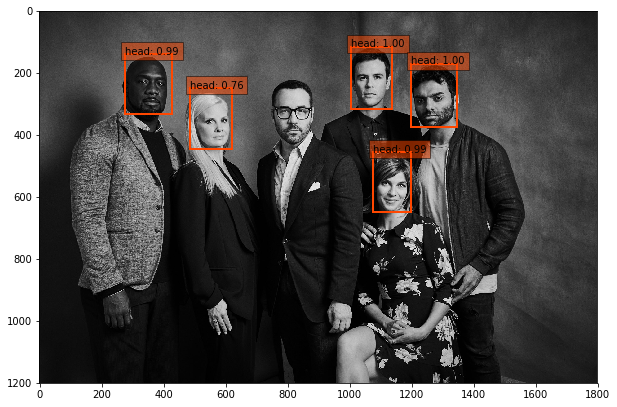
\includegraphics[width=\linewidth]{images/caffessd1.png}
	\caption{Melnbalts attēls, ko izmantoja modeļa pārbaudīšanai ar \textit{SSD} detektēto objektu ierobežojošajiem logiem}
	\endminipage\hfill
	\minipage{0.50\textwidth}%
	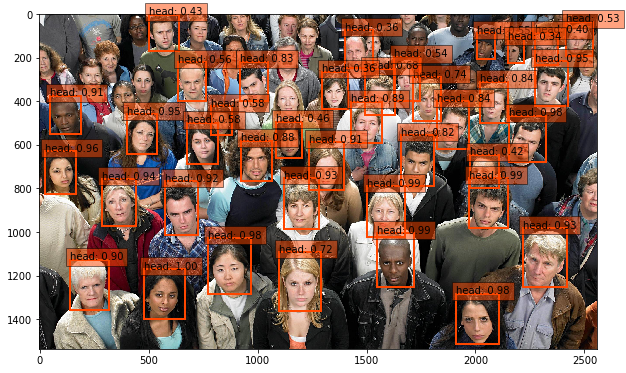
\includegraphics[width=\linewidth]{images/caffessd2.png}
	\caption{Augsta cilvēku blīvuma attēls, ko izmantoja modeļa pārbaudīšanai ar \textit{SSD} detektēto objektu ierobežojošajiem logiem}
	\endminipage
\end{figure}

Gan attēlā 3.1, gan attēlā 3.2 redzamie ierobežojošie logi norāda uz detektēšanas sistēmas atrastajiem objektiem. Minētajos attēlos var novērot, ka detektēšanas sistēma nav atradusi visus iespējamos objektus, bet ir atrasta vismaz lielākā daļa objektu un var pieņemt, ka tīkls ir pietiekami apmācīts, lai to izmantotu gala risinājumā. Kā iemeslus visu objektu neatrašanai var minēt melnbalto krāsu paleti attēlā 3.1 un augsto cilvēku izvietojuma blīvumu attēlā 3.2. 

\paragraph{\textit{YOLO} detektēšanas sistēmas apmācība izmantojot \textit{darknet} ietvaru}
\hfill\par
Pēc datu sagatavošanas, \textit{YOLO} konfigurācijas failos ir jānorāda kura tīkla arhitektūra tiks izmantota (\textit{darknet} piedāvā lielu apjomu ar \textit{YOLO} tīkla arhitektūru variācijām), kurā direktorijā atrodas apmācību dati, klašu skaits un jānorāda direktorija kur atrodas fails ar visu klašu nosaukumiem. Tika izveidoti 3 konfigurācijas faili: 
\begin{enumerate}
	\item norādes uz apmācības datu direktorijām un klašu skaitu; 
	\item visu klašu nosaukumiem;
	\item tīkla arhitektūra, kurā norādīti katra slāņa parametri;
\end{enumerate}

Pirmais minētais fails satur informāciju par klašu skaitu, norādi uz apmācības un validācijas failu apakškopām, norāde uz failu ar visu klašu nosaukumiem un norādi kur glabāt apmācītos modeļus. Šī darba nolūkos šis fails ir ar sekojošu struktūru: 
\begin{lstlisting}
	classes= 1  
	train  = obj/2012_train.txt  
	valid  = obj/2012_test.txt  
	names = cfg/obj.names  
	backup = backup/
\end{lstlisting}

Fails ar visu klašu nosaukumiem ir ļoti vienkāršs, katrā jaunā rindā ir ierakstīts apmācības datos esošo klašu nosaukumi. Šī darba ietvaros šis fails satur tikai vienu ierakstu "head", kas apzīmē datu kopā esošos galvu attēlu piemērus.

Pēdējais minētais fails, ko nepieciešams sagatavot, lai sāktu apmācību ir tīkla arhitektūras konfigurācijas fails. Lai lieki nesarežģītu apmācības procesu, autors izmantoja \textit{darknet} ietvarā piedāvāto noklusējuma konfigurāciju un veica sekojošas izmaiņas:

\begin{enumerate}
	\item \textit{batch} mainīgais konfigurācijā tika nomainīts uz 64, kas apzīmē cik liela attēlu kopa tiks izmantota katrā apmācības solī. Jo lielāku iestata šo vērtību, jo vairāk skaitļošanas resursus prasīs tīkla apmācība.
	\item \textit{subdivision} mainīgais konfigurācijā tika nomainīts uz 4, kas apzīmē, cik daļās tika sadalīta katra pirmajā punktā minētā attēlu kopa, lai izlīdzinātu \textit{GPU} operatīvās atmiņas patēriņu.
	\item \textit{classes} mainīgais konfigurācijā tika nomainīts uz 1, kas apzīmē cik klases tiks detektētas.
	\item \textit{filters} mainīgais pēdējā tīkla slānī tika nomainīts uz 30 pēc formulas $filters=(classes + 5)*5$
\end{enumerate}

Pēdējais solis pirms apmācības sākšanas ir sākuma svaru iegūšana, kas ir publiski pieejami lejupielādei. Pēc sākuma svaru lejupielādēšanas, apmācība var sākties. 

Līdzīgi kā \textit{SSD} gadījumā, arī apmācot \textit{YOLO} detektēšanas sistēmu, lai zinātu, kad pārtraukt apmācību, autors novēroja \textit{mAP} jeb \textit{Mean Average Precision} metriku un \textit{loss} funkcijas atgrieztās vērtības, kad tās sāka tuvoties nullei, regulāri tika pārbaudīti attēli, kuros novērojamas galvas. Kad modelim piedāvātie attēli atgrieza apmierinošas vērtības, autors pieņēma, ka modelis ir pietiekami labi apmācīts, lai to izmantotu gala risinājumā.

\begin{figure}[!htb]
	\minipage{0.50\textwidth}
	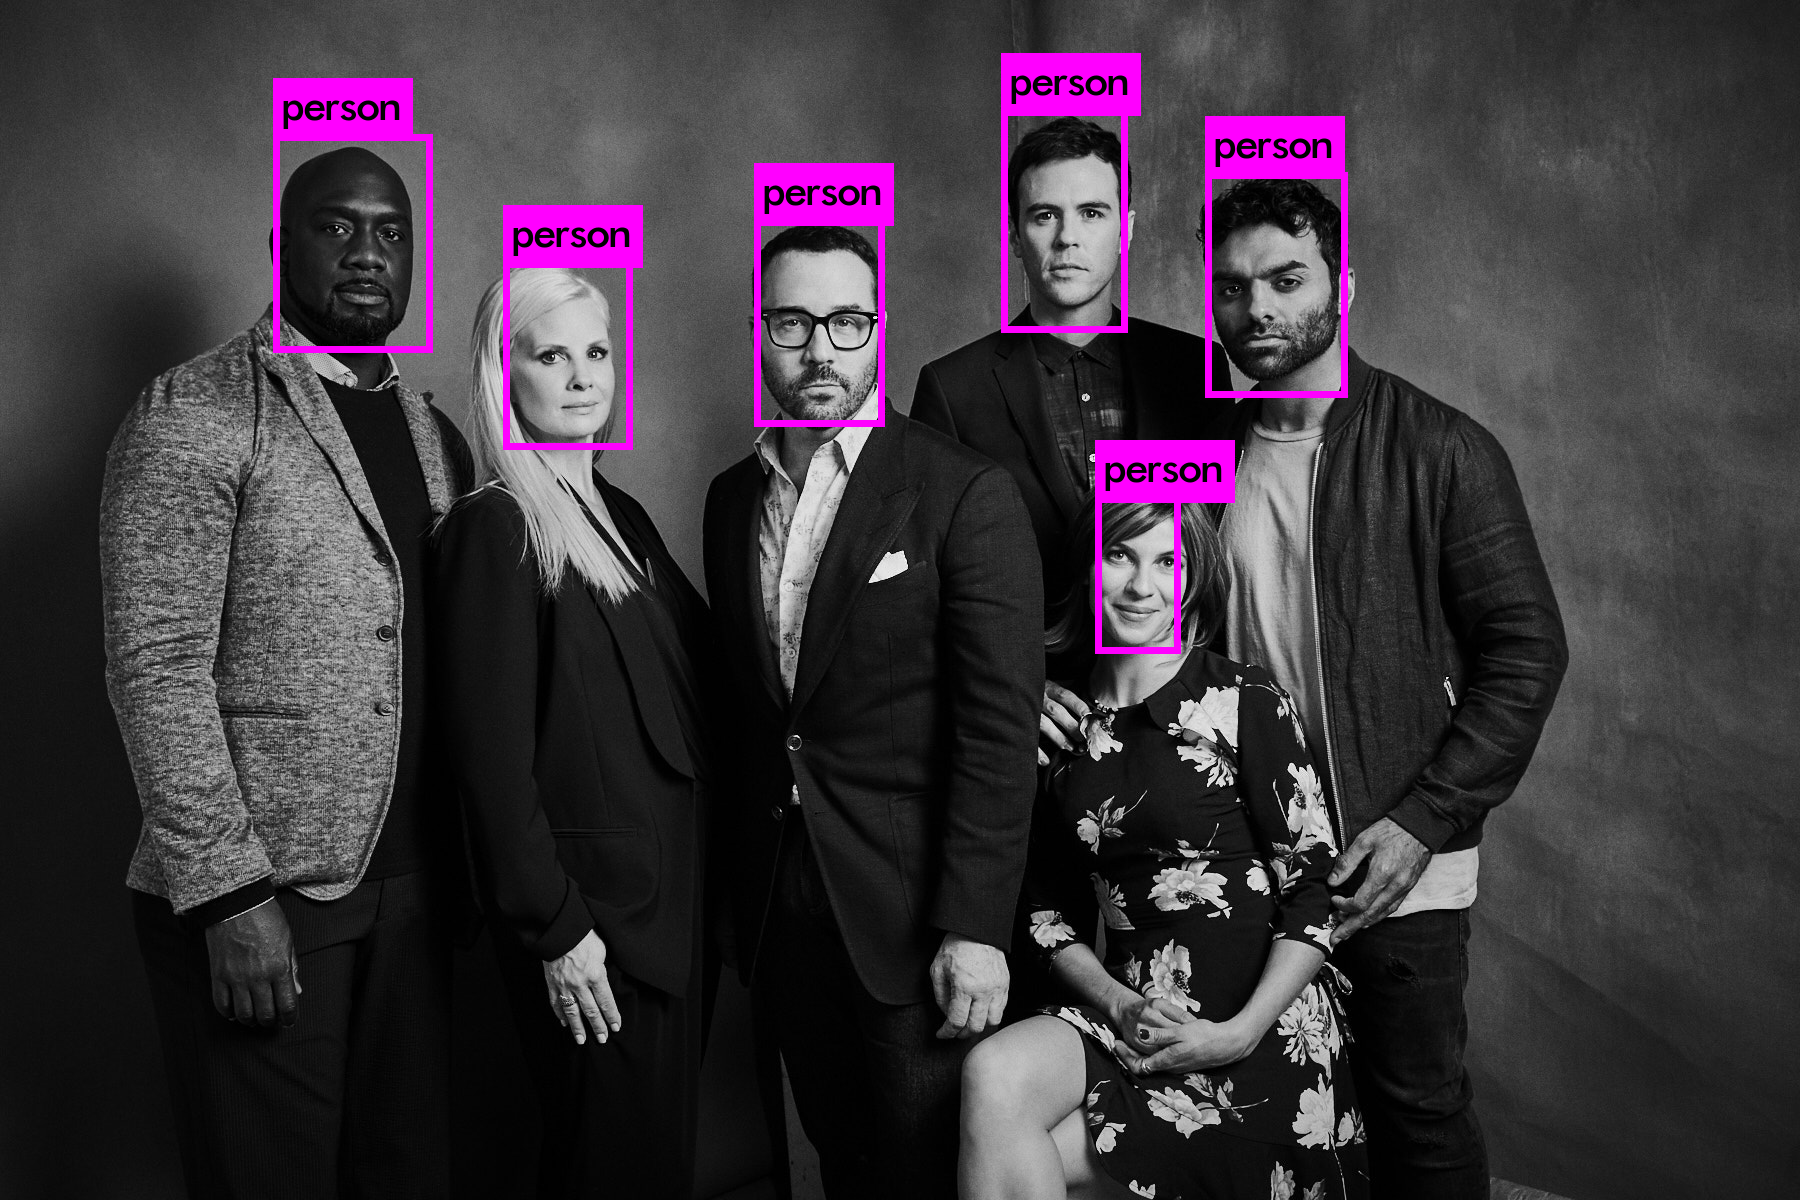
\includegraphics[width=\linewidth]{images/predictions.png}
	\caption{Melnbalts attēls, ko izmantoja modeļa pārbaudīšanai ar \textit{YOLO} detektēto objektu ierobežojošajiem logiem}
	\endminipage\hfill
	\minipage{0.50\textwidth}%
	\includegraphics[width=\linewidth]{images/predictions2.png}
	\caption{Augsta cilvēku blīvuma attēls, ko izmantoja modeļa pārbaudīšanai ar \textit{YOLO} detektēto objektu ierobežojošajiem logiem}
	\endminipage
\end{figure}

Attēlā 3.3, \textit{YOLO} objektu detektēšanas sistēma ir spējusi atrast visus 6 attēlā esošos, interesējošos objektus, kamēr attēlā ar augstu cilvēku blīvumu, detektēšana ir krietni vājāka. Kā iemeslu vājajai detektēšanai attēlos ar augstu cilvēku blīvumu, var minēt \textit{YOLO} algoritma nianses. Režģi, kuros sadala attēlu pārklājas vairākiem objektiem un \textit{YOLO} sagādā problēmas mazu objektu detektēšana. Šo problēmu var daļēji novērst, detektēšanas laikā, padot sistēmai attēlus ar augstāku izšķirtspēju, lai režģu izveidošana attēlam ir vienmērīgāka, taču šāds process tērētu lielākus skaitļošanas resursus. 
\section{Detektēšanas un sekošanas algoritmu implementācija}
Pēc tīkla apmācības gan \textit{caffe}, gan \textit{darknet} ietvars atgriež modeļus ar tīkla svariem. Izmantojot šos modeļus, ir iespējams veikt objektu detektēšanu attēlos. Abi ietvari piedāvā sagatavotas metodes objektu detektēšanai, balstoties uz no apmācības iegūtajiem modeļiem, programmēšanas valodā \textit{Python}. Šīs metodes abiem ietvariem ir pilnīgi atšķirīgas un tās apraksta abu detektēšanas algoritmu darbību. Ja neskaita labojumus, kas tika veikti sakarā ar detektēšanai padoto datu formātu un klašu skaitu, abu ietvaru piedāvātās metodes objektu detektēšanai darbojās un tām nebija nepieciešamas korekcijas. Gan \textit{caffe}, gan \textit{darknet} ietvari piedāvā \textit{detect} funkcijas, implementētas \textit{Python} programmēšanas valodā. Abiem ietvariem šīs funkcijas atgriež visu atrasto objektu ierobežojošo logu koordinātes, klases nosaukumu un ar kādu pārliecību sistēma domā, ka atrastais objekts pieder minētajai klasei. Vienīgā lieta kas mainās šo funkciju atgrieztajos rezultātos ir informācijas formatējums un gala risinājuma implementāciju tas ļoti neietekmē. Ņemot vērā minēto informāciju, var secināt, ka pēc detektēšanas posma, pārējā risinājuma implementācija abām detektēšanas sistēmām būs vienāda. Lai izvairītos no atkārtošanās, šīs sadaļas ietvaros tiks apskatīta tikai \textit{SSD} detektēšanas sistēmas un dažādu sekošanas algoritmu apvienošana vienā risinājumā.
\paragraph{Sekošana pēc detektēšanas ar \textit{OpenCV} bibliotēkā piedāvātajiem risinājumiem} //TODO, jāpievieno par LOI un skaitīšanu 
\hfill\par
\textit{OpenCV} ir atvērtā koda datorredzes un mašīnmācīšanās programmatūras bibliotēka, kurā ir implementēti arī divi no trim darbā apskatītajiem sekošanas algoritmiem: \textit{MIL} jeb \textit{Multiple Instance Learning} un \textit{AdaBoost} sekošanas algoritmi. Pirmais solis sekošanas risinājuma izveidē ir video interesējošā reģiona izvēlēšanās (ir iespējams izvēlēties, ka detektēšana un sekošana nenotiek visā video laukumā, bet tikai daļā no video) un sekotāja (no angļu val. \textit{tracker}) uzstādīšana. Kad tas izdarīts, tiek atvērts video fragments un detektēšanas algoritms apskata vienu kadru pēc otra, līdz atrasts kāds no interesējošajiem objektiem, šajā gadījumā cilvēku galvas. Kad detektēšanas sistēma ir atradusi objektu, no objekta koordinātēm tiek izveidots ierobežojošais logs, tas tiek parādīts un notiek sekotāja inicializēšana šajā ierobežojošajā logā. Nākamajos kadros no jauna notiek objektu detektēšana un jaunu sekotāju inicializēšana un tiek atjaunotas iepriekšējos kadros izveidoto sekotāju atrašanās vietas.  

Papildus dažādu sekošanas algoritmu implementācijām, \textit{OpenCV} programmatūras bibliotēka piedāvā arī metodes, kas var atvieglo darbu ar attēliem un video fragmentiem.  
\begin{lstlisting}[language=Python]
roi = cv2.selectROI(firstFrame,False)
tracker = cv2.MultiTracker_create()   
while(videoFile.isOpened()):  
	ret, frame = videoFile.read()     
	result = detection.detect(frame)    
\end{lstlisting}
Šajā koda fragmentā ir atlasītas svarīgas inicializācijas metodes. Šajās koda rindās uzskaitītas metodes, kas inicializē reģionu kurā veiks detektēšanu un sekošanu. Tiek inicializēts \textit{OpenCV} piedāvātais \textit{MultiTracker} objekts \cite{multitrack}, kas ļauj vienlaikus uzturēt vairākus aktīvus sekotājus. Ciklā tiek atvērts video fragments un atlasīts kadrs, kuram veic detektēšanas operāciju. Nākamās koda rindas darbojas ar detektēšanas procesā atrastajiem objektiem.

\begin{lstlisting}[basicstyle=\tiny]
detectCenter = (int((xmin + xmax)*0.5),int((ymin+ymax)*0.5))   
if (roi[1] < detectCenter[1] < roi[1]+roi[3] and roi[0] < detectCenter[0] < roi[0]+roi[2]):
	cv2.rectangle(frame,(xmin, ymin), (xmax, ymax),(255, 0, 0),3)            
	cv2.putText(frame,item[-1] + str(item[-2]),(xmin,ymin), font, 0.5,(255,255,255),2,cv2.LINE_AA)                   
	if not boxCenters:
		tracker.add(cv2.TrackerMIL_create(), frame, bbox)
	else:
		newTracker = False
		distanceList = list()
		for cent in boxCenters:
			distanceList.append(math.sqrt( ((cent[0]-detectCenter[0])**2)+((cent[1]-detectCenter[1])**2)))
		if min(distanceList)>100:
			newTracker = True
	if newTracker:
		tracker.add(cv2.TrackerMIL_create(), frame, bbox)
ok, boxes = tracker.update(frame)
\end{lstlisting} 
\chapter{Rezultāti}

Lai gan ierobežotu skaitļošanas resursu dēļ abu darbā apskatīto detektēšanas sistēmu konvolūcijas neironu tīklu apmācība tika veikta ļoti neilgu laiku (aptuveni nedēļu), iegūtie rezultāti ir apmierinoši kā pamats nopietnākas cilvēku plūsmas analīzes sistēmas izstrādei. Darba izstrādes laikā autoram neizdevās praktiski implementēt \textit{SiamFC} sekošanas algoritmu, kas ir balstīts uz vairākiem neironu tīkliem un potenciāli varētu krietni uzlabot iegūtos rezultātus. Veidojot rezultātus, tiks salīdzināta objektu sekošana 3 dažādos video fragmentos ar 2 dažādām objektu detektēšanas sistēmām un 2 dažādiem sekošanas algoritmiem. Pēc abu detektēšanas sistēmu apmācības pirmie rezultāti, ko salīdzināt ir tīklu precizitātes metrika \textit{mAP}. \textit{Caffe} ietvarā \textit{SSD} detektēšanas sistēmai precizitāti var aprēķināt ietvara direktorijā izsaucot komandu \textit{"python examples/ssd/score_ssd_pascal.py"}, šī komanda atgrieza vērtību 71\%. \textit{Darknet} ietvarā \textit{YOLO} detektēšanas sistēmai precizitāti var aprēķināt ietvara direktorijā izsaucot komandu\textit{ "./darknet detector map data/obj.data cfg/yolo-obj.cfg backup/yolo-obj_24900.weights"}, šī komanda atgrieza vērtību 75\%. 

Salīdzinot \textit{MIL} un \textit{AdaBoost} sekošanas algoritmus, \textit{MIL} algoritms strādāja daudz lēnāk un tērēja vairāk skaitļošanas resursu, kamēr \textit{AdaBoost} algoritms bija daudz ātrāks, taču nebija tik precīzs.

\paragraph{\textit{SSD} detektēšanas sistēma ar \textit{OpenCV} sekošanas algoritmiem}
\hfill\par

Apmācībai \textit{SSD} detektēšanas sistēmai ievades dati tika padoti izmērā 512x512 pretēji standarta 300x300. Palielinot šo izšķirtspēju tiek upurēts apmācības ātrums, taču iespējams iegūt precīzākus rezultātus. Darba turpinājumā tiks apskatīti \textit{MIL} sekošanas algoritma rezultāti. 
 
\begin{figure}[h]%
	\centering
	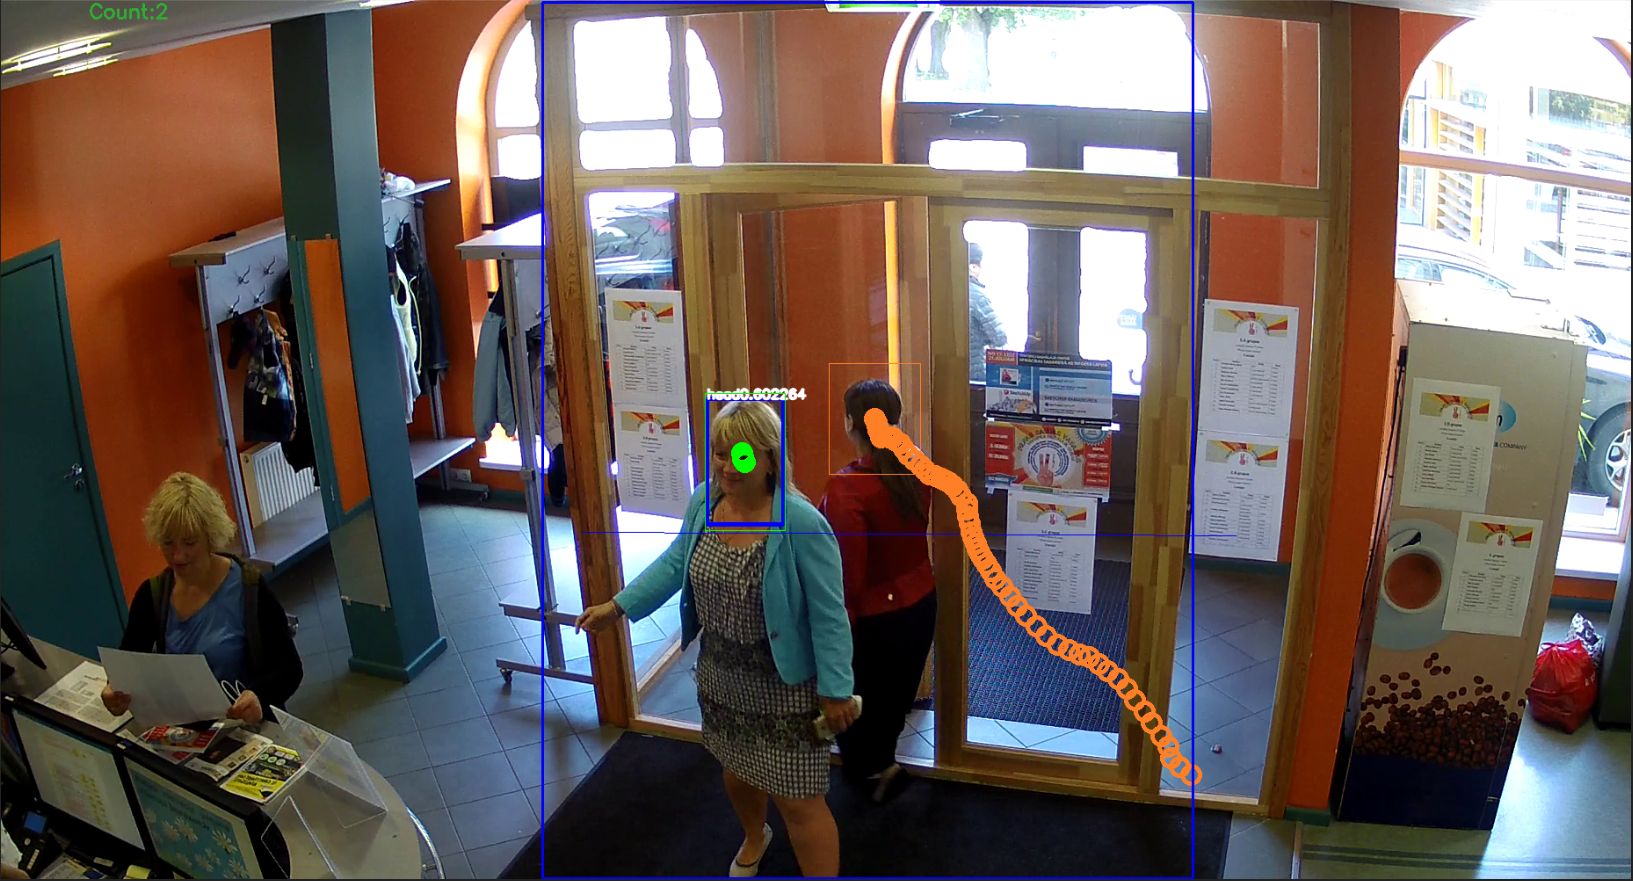
\includegraphics[height=6cm]{images/ssd1.png} %
	\caption{\textit{SSD} detektēšanas sistēma ar \textit{MIL} sekošanas algoritmu. Pirmais video.}%
	\label{fig:example}%
\end{figure}
\newpage
Attēlā 4.1. ar zilu krāsu atzīmēts sekošanas algoritmam interesējošais reģions. Ar oranžo krāsu atzīmētais ceļš norāda, ka sieviete attēla labajā pusē ir uztverta uzreiz kā sasniegts interesējošais reģions, taču ar zaļo krāsu atzīmētā sieviete ir uztverta vēlu. Vēlamais rezultāts ar zaļo krāsu atzīmēto sievieti uztvertu uzreiz kā tā parādītos durvīs, šajā gadījumā, detektēšana sievieti atradusi pāris kadrus vēlāk kā vēlams. Ir iespējams konfigurēt detektēšanas sistēmu, lai uztvertu objektus ar zemāku pārliecības slieksni, bet tas var izraisīt kļūdainus rezultātus, piemēram, atzīmēt cilvēku kāju kā galvu.

\begin{figure}[h]%
	\centering
	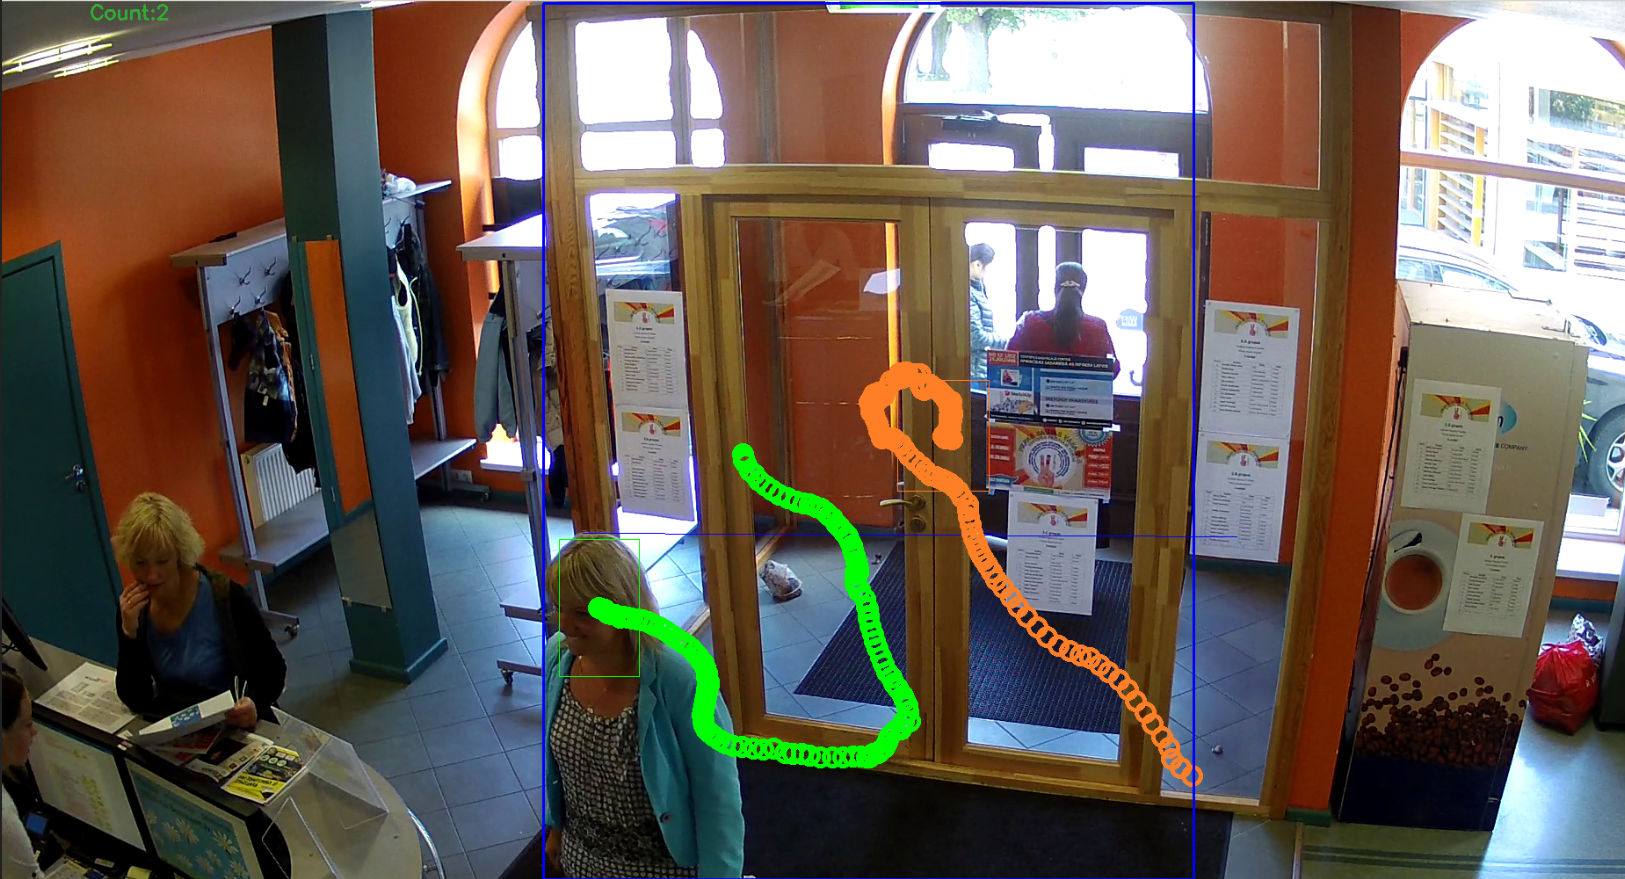
\includegraphics[height=6cm]{images/ssd2.png} %
	\caption{\textit{SSD} detektēšanas sistēma ar \textit{MIL} sekošanas algoritmu. Pirmais video.}%
	\label{fig:example}%
\end{figure}

Attēlā 4.2. attēlots brīdis pāris sekundes vēlāk, kad sieviete, kas attēlā 4.1. bija atzīmēta ar oranžo krāsu jau pametusi telpu, bet sekotājs apstājies pie durvīm. No tā var secināt, ka objektam pazūdot no sekošanas algoritma redzes loka, sekošanas algoritms pazaudē objektu un vairs nespēj to atrast. \textit{OpenCV} sekošanas programmējamā interfeisā piedāvātās metodes šādā brīdī nenorāda, ka objekts pazudis, bet uzskata, ka joprojām ir atrasts. Ar zaļo krāsu atzīmētajai sievietei, sekošanas algoritms ir veiksmīgi izsekojis līdz attēlā norādītajai atrašanās vietai, jo viņas ceļā nav bijuši šķēršļi. Vērts piebilst, ka dotais video fragments ir ļoti augstas izšķirtspējas, kas ļauj veikt objektu detektēšanu ar augstāku precizitāti. 

\begin{figure}[h]%
	\centering
	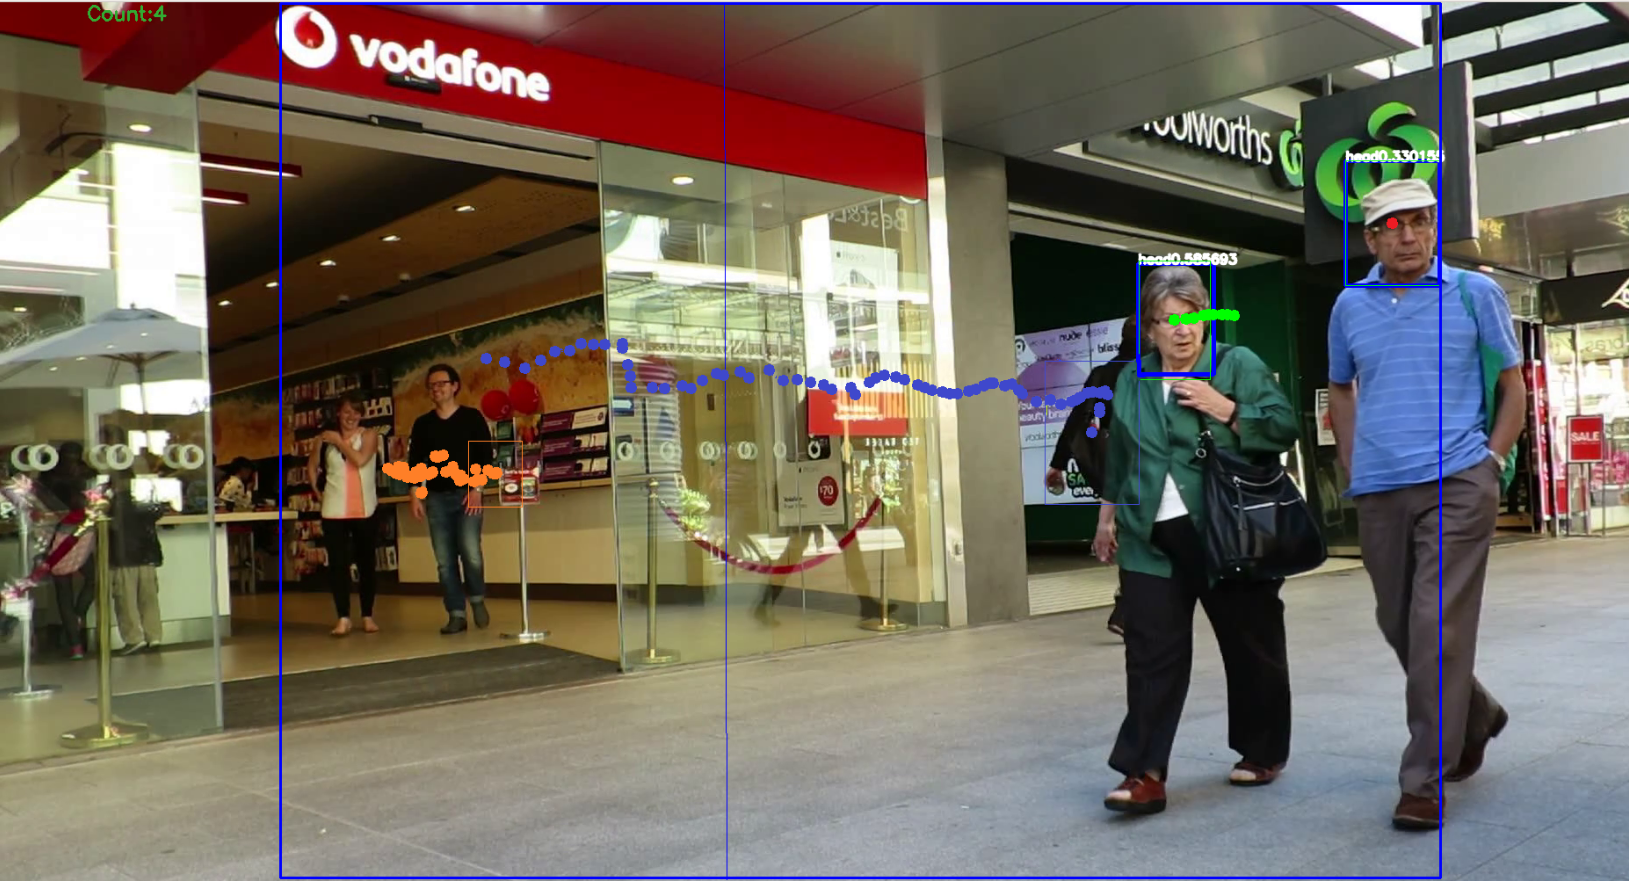
\includegraphics[height=6cm]{images/ssd3.png} %
	\caption{\textit{SSD} detektēšanas sistēma ar \textit{MIL} sekošanas algoritmu. Otrais video.}%
	\label{fig:example}%
\end{figure}

Attēlā 4.3. ir attēlots fragments no cita video, kas ir zemākas izšķirtspējas un filmēts citā vidē. Līdz dotajam brīdim, video fragmentā uztverti 4 objekti, kamēr 1 objekts no visiem nav atrasts. Ar oranžo,violeto un zaļo krāsu atzīmētie objekti ir uztverti pāris kadrus pēc tam, kad tie parādījušies interesējošajā reģionā, kamēr ar sarkano krāsu atzīmētais objekts uztverts uzreiz. Arī šajā gadījumā ir iespējams konfigurēt detektēšanas sistēmu, lai uztvertu objektus ar zemāku pārliecības slieksni, bet tas var izraisīt kļūdainus rezultātus, piemēram, atzīmēt cilvēku kāju kā galvu.

\begin{figure}[h]%
	\centering
	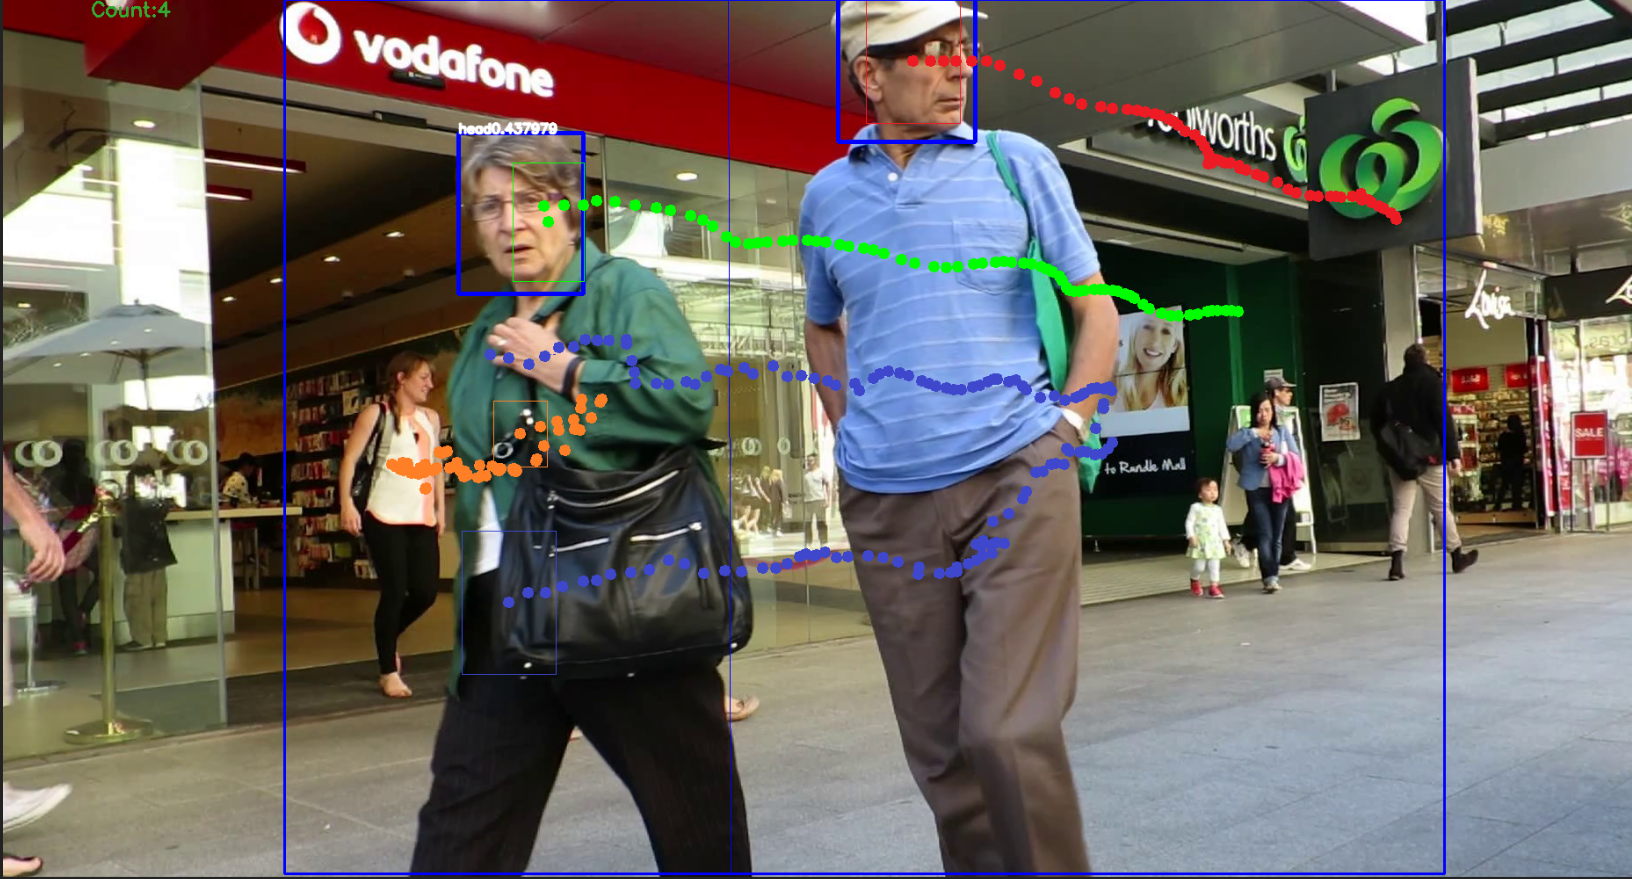
\includegraphics[height=6cm]{images/ssd4.png} %
	\caption{\textit{SSD} detektēšanas sistēma ar \textit{MIL} sekošanas algoritmu. Otrais video.}%
	\label{fig:example}%
\end{figure}

Līdz attēlā 4.4. redzamajam brīdim objektiem, kas ir tuvu filmēšanas punktam ir veiksmīgi izsekots, kamēr vīrietis, kas bija atzīmēts ar violeto krāsu vairs netiek uztverts un priekšplānā esošie objekti, šķērsojot to, lika sekošanas algoritmam kļūdīties un violetajam objektam atkal parādoties vairs nespēja tam izsekot. 

\begin{figure}[h]%
	\centering
	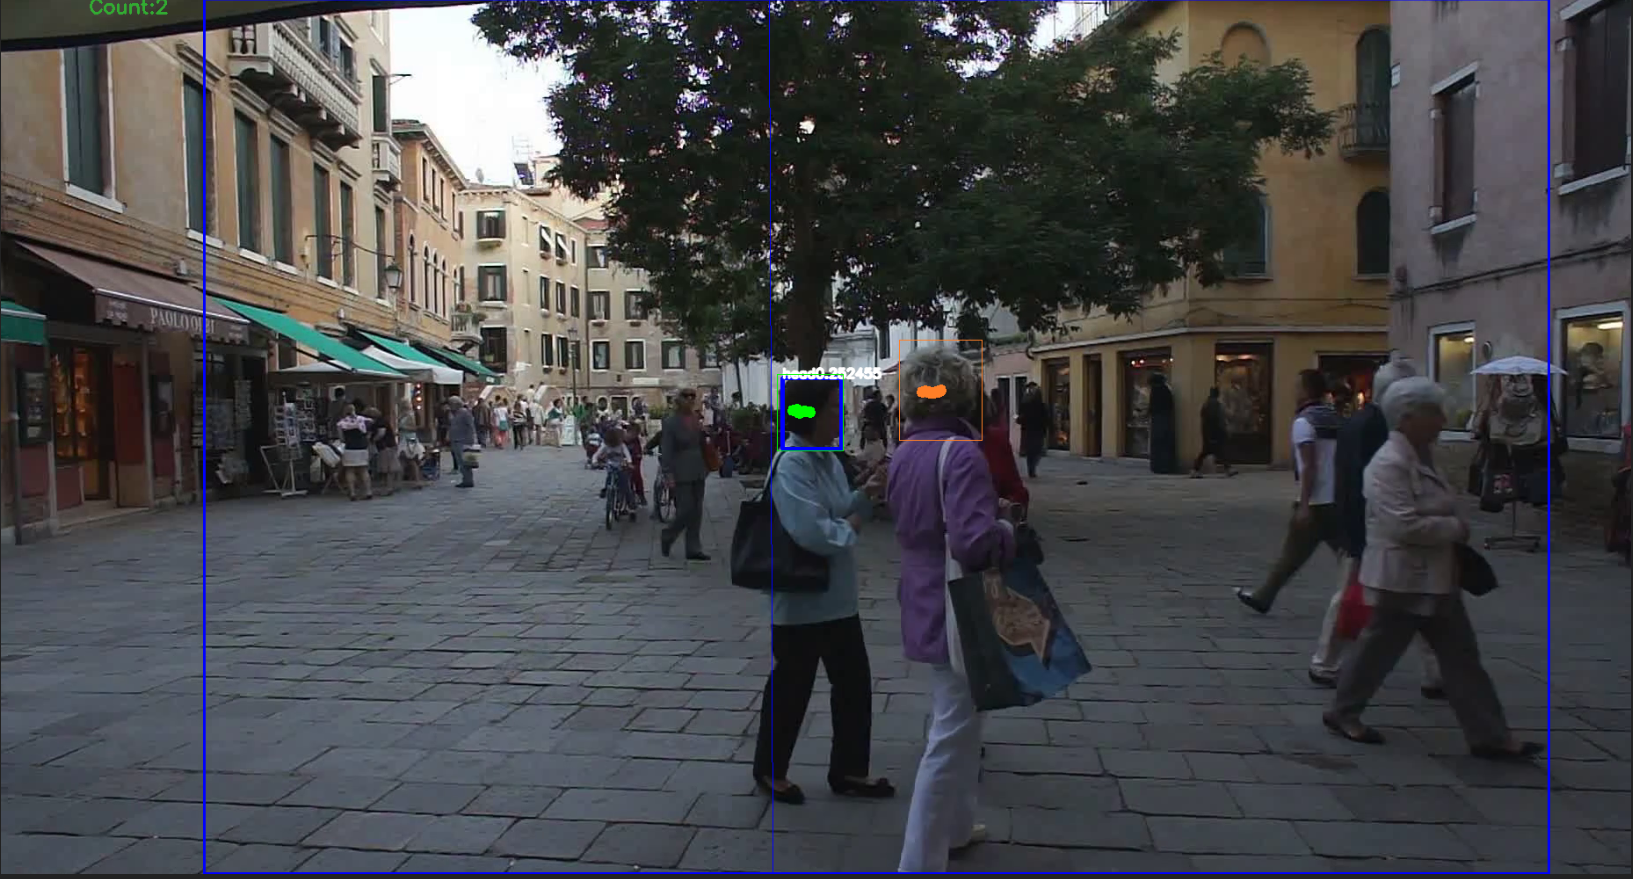
\includegraphics[height=6cm]{images/ssd5.png} %
	\caption{\textit{SSD} detektēšanas sistēma ar \textit{MIL} sekošanas algoritmu. Trešais video.}%
	\label{fig:example}%
\end{figure}

Attēlā 4.5. ir attēlots fragments no cita video, kas ir ļoti zemas izšķirtspējas un filmēts citā vidē. Dotais fragments ir pirmie video kadri, attēlā ir redzami daudz cilvēki, taču detektēšanas algoritms ir atradis tikai divus. Par iemeslu var uzskatīt ļoti zemo video fragmenta izšķirtspēju.

\begin{figure}[h]%
	\centering
	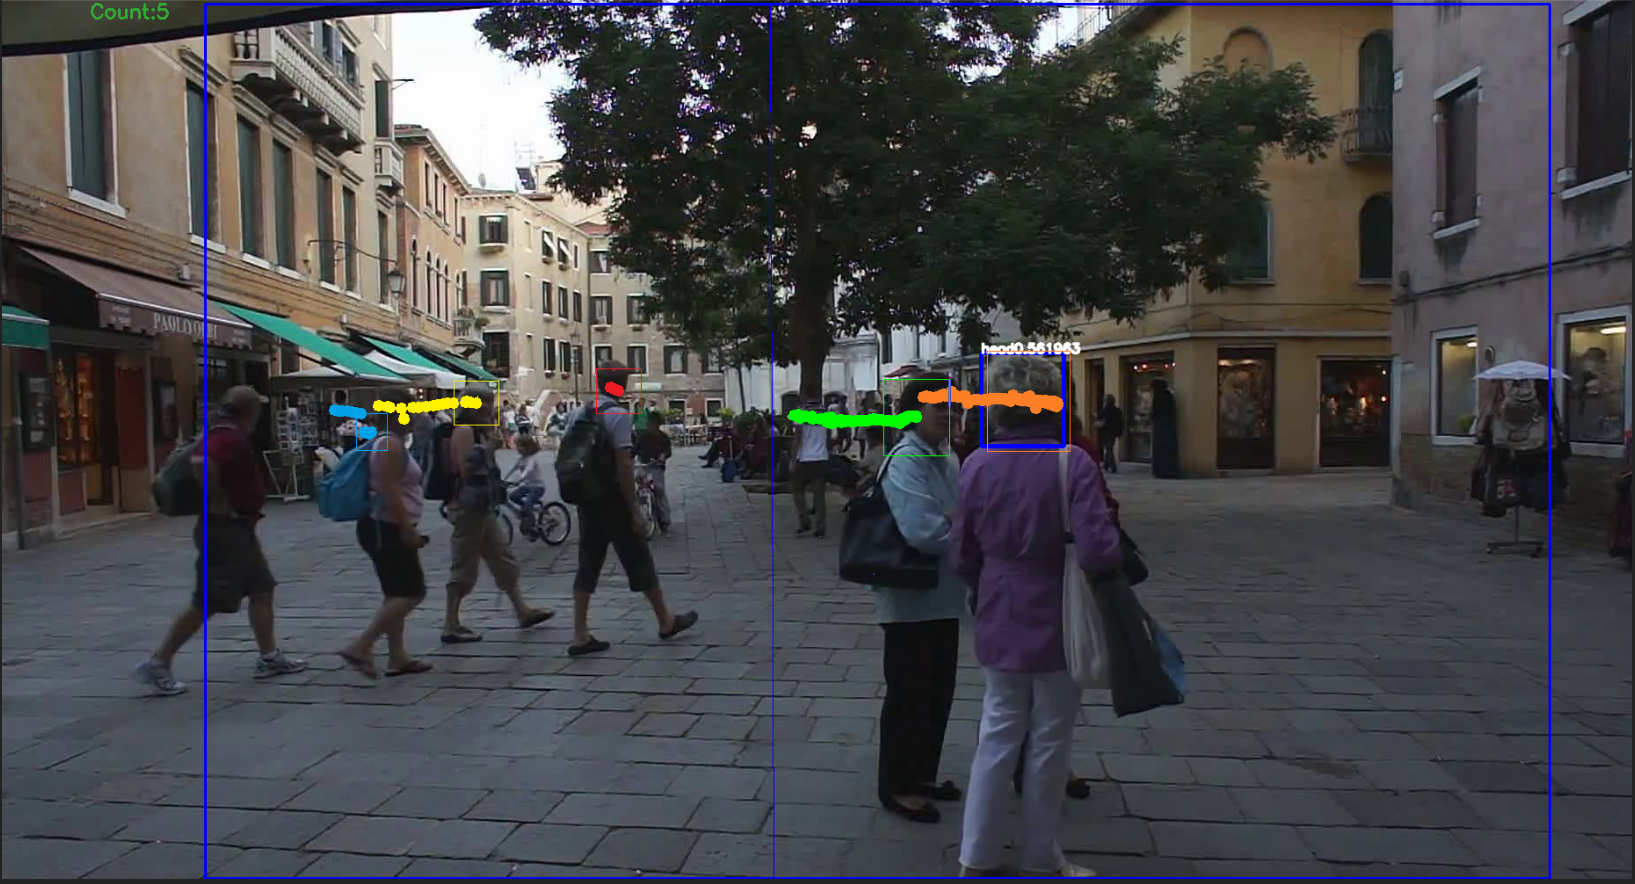
\includegraphics[height=6cm]{images/ssd6.png} %
	\caption{\textit{SSD} detektēšanas sistēma ar \textit{MIL} sekošanas algoritmu. Trešais video.}%
	\label{fig:example}%
\end{figure}

Attēlā 4.6. ir attēlots brīdis no tā paša video, pāris sekundes vēlāk, kad rāmī ir parādījušies un uztverti 3 jauni objekti. Detektēšana gan tiem nav notikusi līdz ar parādīšanos interesējošajā reģionā, bet pāris kadrus vēlāk. 

\textit{AdaBoost} sekošanas algoritms strādā gandrīz tik pat labi kā \textit{MIL} algoritms, brīžiem gan novērojami iztrūkumi, sekošanas laikā sekotājs brīžiem pazaudē objektu, bet ātri, pēc pāris kadriem, to atrod. Līdzīgi kā \textit{MIL} algoritmam, arī \textit{AdaBoost} netiek galā ar objektiem, kas video fragmentos novietojas aiz šķēršļiem, bet izpildes laikā ir ātrāks. Ja gala risinājumā nepieciešams izvēlēties starp \textit{MIL} un \textit{AdaBoost}, autors izvēlētos \textit{MIL}, jo, lai gan \textit{AdaBoost} ir nedaudz ātrāks, \textit{MIL} algoritms objektiem seko stabilāk.
\begin{figure}[h]%
	\centering
	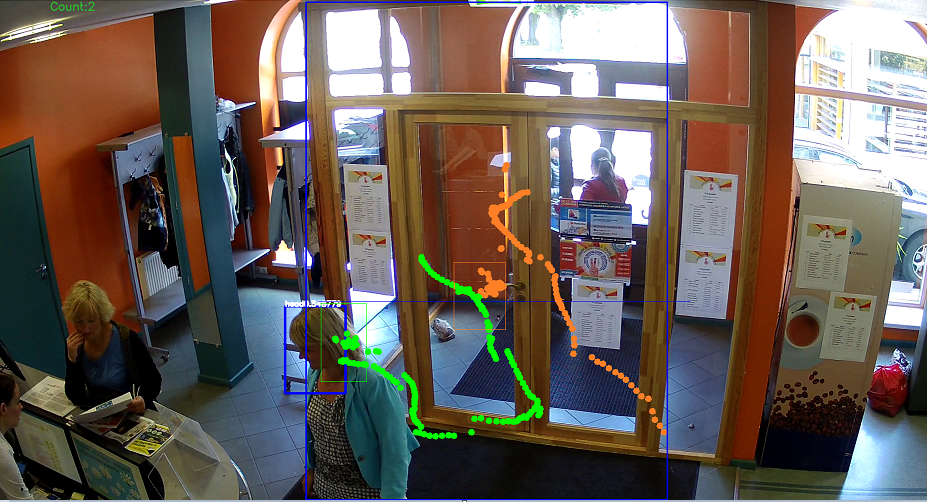
\includegraphics[height=6cm]{images/ssd7.png} %
	\caption{\textit{SSD} detektēšanas sistēma ar \textit{AdaBoost} sekošanas algoritmu. Pirmais video.}%
	\label{fig:example}%
\end{figure}
\paragraph{\textit{YOLO} detektēšanas sistēma ar \textit{OpenCV} sekošanas algoritmiem}
\hfill\par
Salīdzinot ar darba izstrādes laikā apmācīto \textit{SSD} objektu detektēšanas sistēmu, \textit{YOLO} detektēšanas sistēma tika apmācīta krietni mazāku laiku, kas arī atspoguļojās rezultātos. Augstas izšķirtspējas nekustīgos attēlos \textit{YOLO} detektēšanas sistēma rādīja labus rezultātus, taču video fragmentos detektēšanas kvalitāte bija zemāka kā \textit{SSD} detektēšanas sistēmai. Vēl viens iemesls salīdzinoši sliktākajai detektēšanas kvalitātei varētu būt praktiskā implementācija. Implementējot detektēšanu \textit{darknet} ietvarā, grūtības sagādāja no video fragmenta iegūto kadru pārveidošana uz \textit{darknet} \textit{Image} objektu. Tāda iemesla dēļ, pirms veikt detektēšanu, video fragmenti tika sadalīti attēlos un detektēšana tika veikta katram attēlam atsevišķi nevis \textit{OpenCV VideoFile} objektam kā \textit{SSD} gadījumā. Tādā veidā, sekošanas algoritms var pazaudēt savienojumus starp video kadriem.
\newpage
\begin{figure}[H]%
	\centering
	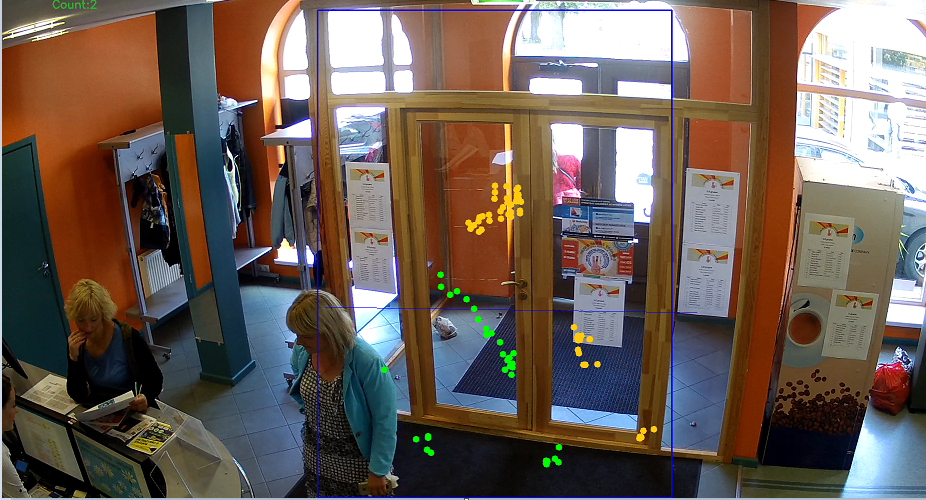
\includegraphics[height=5cm]{images/yolo1.png} %
	\caption{\textit{YOLO} detektēšanas sistēma ar \textit{AdaBoost} sekošanas algoritmu. Pirmais video.}%
	\label{fig:example}%
\end{figure}
\begin{figure}[H]%
	\centering
	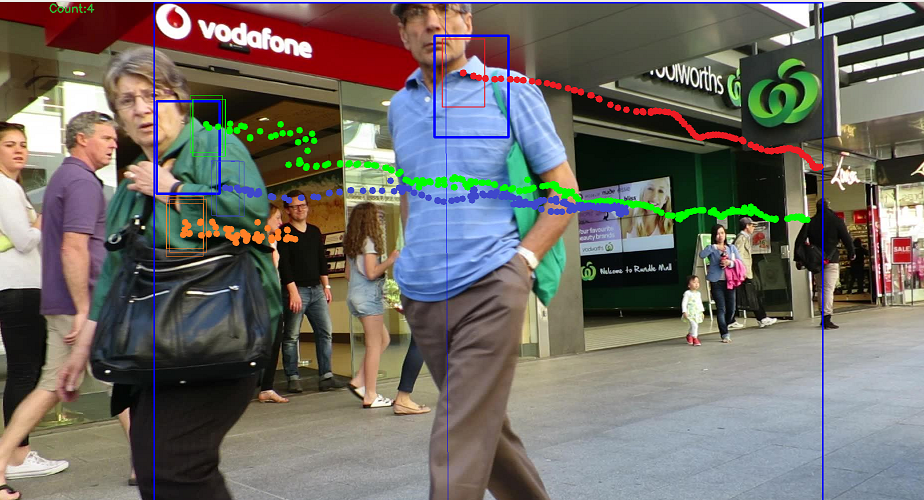
\includegraphics[height=5cm]{images/yolo2.png} %
	\caption{\textit{YOLO} detektēšanas sistēma ar \textit{AdaBoost} sekošanas algoritmu. Otrais video.}%
	\label{fig:example}%
\end{figure}
\begin{figure}[H]%
	\centering
	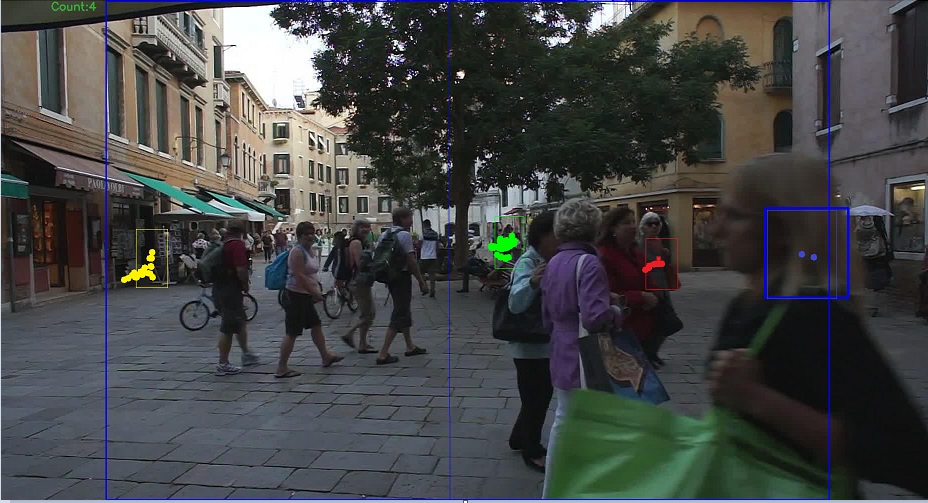
\includegraphics[height=5cm]{images/yolo3.png} %
	\caption{\textit{YOLO} detektēšanas sistēma ar \textit{AdaBoost} sekošanas algoritmu. Trešais video.}%
	\label{fig:example}%
\end{figure}
\newpage
Attēlā 4.8. var novērot, ka sekojot rodas iztrūkumi un detektēšana ir darbojusies līdzīgi \textit{SSD} detektēšanas sistēmai. Attēlā 4.9. priekšplānā esošie cilvēki ir detektēti labāk kā \textit{SSD} sistēmai, taču fonā esošie netiek atrasti. Kā jau darbā minēts, \textit{YOLO} slikti detektē mazus objektus, kas varētu būt iemesls. Sekošanas algoritms attēlā 4.9. darbojas līdzīgi kā \textit{MIL} sekošanas algoritms, kur objekti, aizklājot citus, pārtvēra to ierobežojošos logus. 

Tā kā video fragments attēlā 4.10. ir ļoti zemas izšķirtspējas, visi objekti ir salīdzinoši mazi, kas \textit{YOLO} sagādā lielas problēmas. Fona esošais objekts ir atrasts veiksmīgi, bet pārējie cilvēki, kas pārvietojas fonā tiek detektēti ļoti vāji.
\chapter{Secinājumi un priekšlikumi}
\paragraph{Secinājumi}
\hfill\par
\begin{enumerate}
	\item Jaunākie risinājumi balss atpazīšanā, objektu klasifikācijā un objektu detektēšanā ir veidoti izmantojot dziļās mašīnmācīšanās metodes.
	\item Konvolūcijas neironu tīkli vislabāk risina detektēšanas, segmentācijas un klasifikācijas problēmas.
	\item \textit{VGG Net} konvolūcijas neironu tīklu arhitektūra ir labi optimizēta, lai nebūtu nepieciešami ļoti lieli skaitļošanas resursi, tai pat laikā atgriežot kvalitatīvus rezultātus.
	\item Jo vairāk konvolūcijas slāņu (filtru) neironu tīklā, jo labāk šis tīkls veiks klasifikāciju, taču vairāk slāņu izmantošana nozīmē papildu skaitļošanas jaudas nepieciešamību.
	\item Lai efektīvi darbotos ar konvolūciju neironu tīkliem, apmācību ir nepieciešams veikt, izmantojot grafisko procesoru, kam ir daudz vairāk skaitļošanas vienības kā centrālajiem procesoriem.
	\item Dotajā brīdī, \textit{ReLU} ir labākā konvolūciju neironu tīklos izmantotā aktivizācijas funkcija. 
	\item Izveidot savu konvolūcijas neironu tīklu arhitektūru ir viegli, taču, lai to padarītu labāku par jau eksistējošajām arhitektūrām, ir nepieciešams ieguldīt daudz laika pētījumos un eksperimentos.
	\item Izvēloties programmatūras ietvarus darbam ar konvolūcijas neironu tīkliem ir pieejami daudz varianti, taču, lai izvēlētos īsto ir svarīgs gala risinājuma mērķis. Piemēram, \textit{Caffe} ir speciāli veidots darbam ar konvolūcijas neironu tīkliem un \textit{darknet} satur oriģinālo \textit{YOLO} implementāciju. 
	\item Uz reģionu priekšlikumiem balstītās detektēšanas metodes var efektīvi izmantot, ja apmācībai ir pieejamas ierīces ar augstu skaitļošanas jaudu.
	\item \textit{YOLO} ir ļoti ātra objektu detektēšanas sistēma.
	\item \textit{SSD} detektēšanas sistēma ir labākais detektēšanas precizitātes un ātruma kompromiss.
	\item Izmantojot augstas izšķirtspējas attēlus, apmācības laikā, var uzlabot detektēšanas sistēmas veiktspēju, taču tiek upurēti skaitļošanas resursi.
	\item Objektu sekošanas algoritmus ir nepieciešams implementēt, lai nepazaudētu objektu, kad detektēšanas sistēmas vairs nevar to atrast.
	\item Jo lielāka apmācības datu kopa, jo dažādākus objektus detektēšanas sistēmas var atrast.
	\item Nepopulāras datu kopas (datu kopas, kas nav \textit{Pascal VOC, MS COCO, ILSVRC}) pielietotu ar populārākajiem konvolūcijas neironu tīklu programmatūras ietvariem, var nākties veikt datu pārveidojumus kā anotāciju formāta maiņu.
	\item \textit{Python} programmēšanas valodā ir pieejamas daudz un dažādas datorredzes un mašīnmācīšanās programmatūras bibliotēkas. Šīs programmatūras bibliotēkas kā arī elementārā koda sintakse padara \textit{Python} programmēšanas valodu viegli izmantojamu, lai darbotos dziļās apmācības laukā.
	\item Lai sasniegtu labākus detektēšanas sistēmu rezultātus, konvolūcijas neironu tīklu apmācība ir jāveic daudz ilgāk kā šī darba ietvaros.
	\item \textit{AdaBoost} sekošanas algoritms darbojās ātrāk kā \textit{MIL}, taču \textit{MIL} algoritms uzrādīja labākus rezultātus.
	\item Šī darba ietvaros praktiski implementētie sekošanas algoritmi nespēja atrast objektus, kad tie pazūd fonā aiz priekšplānā esošajiem objektiem.
	\item Ja video fragments ir augstas izšķirtspējas un uzņemts ar kameru no paaugstināta skatu punkta, kur skaitīšanas līniju var novietot horizontāli un cilvēki pārvietojas vertikāli, tad, šī darba ietvaros izveidotais risinājums, teorētiski, būtu labi funkcionējošs.
\end{enumerate}
\paragraph{Priekšlikumi}
\hfill\par
\begin{enumerate}
	\item Lai uzlabotu šī darba ietvaros izveidoto sistēmu, ir nepieciešams abas izmantotās detektēšanas sistēmas apmācīt ilgāk. Izmantotajā datu kopā ir vairāk kā 220 tūkstoš attēlu un šī darba ietvaros veiktās apmācības ilgums ir nepietiekams, lai iegūtu labākus rezultātus ar attēliem, kas nav no datu kopas.
	\item Lai iegūtu labākus detektēšanas rezultātus un, pieņemot, ka ir pieejami neierobežoti skaitļošanas resursi, šī darba ietvaros \textit{VGG Net} konvolūcijas neironu tīklu arhitektūru būtu vērtīgi aizstāt ar \textit{ResNet} konvolūcijas neironu tīklu arhitektūru. \textit{ResNet} arhitektūra satur daudz vairāk slāņus un labāk detektē objektus, bet apmācība pieprasa augstu skaitļošanas jaudu. 
	\item Lai uzlabotu sekošanas algoritmu veiktspēju, var izmantot uz konvolūcijas neironu tīklu apmācību balstītus sekošanas algoritmus. Darbā minētais \textit{SiamFC} ir viena no šādām sistēmām, kuru gan darba izstrādes laikā neizdevās praktiski implementēt. Papildu detektēšanas sistēmu apmācībai, nākamais solis risinājuma izstrādē būtu pielietot \textit{SiamFC} sekošanas sistēmu. 
\end{enumerate} 
\bibliographystyle{ieeetr}
\selectlanguage{latvian}
\bibliography{src/links,src/articles,src/books}	%to load the *.bib files ../articles,../books,
\addcontentsline{toc}{chapter}{Izmantotās literatūras un avotu saraksts}

\label{LastPage}

%% Te vajadzētu pielikumus
\appendix
\chapter{Pirmais pielikums}
\label{appendix:pielikums1}
\begin{lstlisting}[basicstyle=\tiny]
cur_dir=$(cd $( dirname ${BASH_SOURCE[0]} ) && pwd )
root_dir=$cur_dir/../..
cd $root_dir
redo=1
data_root_dir="$HOME/data/VOCdevkit"
dataset_name="VOC0712"
mapfile="$root_dir/data/$dataset_name/labelmap_voc.prototxt"
anno_type="detection"
db="lmdb"
min_dim=0
max_dim=0
width=0
height=0
extra_cmd="--encode-type=jpg --encoded"
if [ $redo ]
then
extra_cmd="$extra_cmd --redo"
fi
for subset in test trainval
do
python $root_dir/scripts/create_annoset.py --anno-type=$anno_type --label-map-file=$mapfile --min-dim=$min_dim --max-dim=$max_dim --resize-width=$width --resize-height=$height --check-label $extra_cmd $data_root_dir $root_dir/data/$dataset_name/$subset.txt $data_root_dir/$dataset_name/$db/$dataset_name"_"$subset"_"$db examples/$dataset_name
\end{lstlisting}
\addtocounter{nofappendices}{1}
\chapter{Otrais pielikums}
\label{appendix:pielikums2}
\begin{lstlisting}[basicstyle=\tiny]
import xml.etree.ElementTree as ET
import pickle
import os
from os import listdir, getcwd
from os.path import join
sets=[('2007', 'train'), ('2007', 'val'), ('2007', 'test')]
classes = ["head"]
def convert(size, box):
dw = 1./(size[0])
dh = 1./(size[1])
x = (box[0] + box[1])/2.0 - 1
y = (box[2] + box[3])/2.0 - 1
w = box[1] - box[0]
h = box[3] - box[2]
x = x*dw
w = w*dw
y = y*dh
h = h*dh
return (x,y,w,h)
def convert_annotation(year, image_id):
in_file = open('VOCdevkit/VOC%s/Annotations/%s.xml'%(year, image_id))
out_file = open('VOCdevkit/VOC%s/labels/%s.txt'%(year, image_id), 'w')
tree=ET.parse(in_file)
root = tree.getroot()
size = root.find('size')
w = int(size.find('width').text)
h = int(size.find('height').text)
for obj in root.iter('object'):
difficult = obj.find('difficult').text
cls = obj.find('name').text
if cls not in classes or int(difficult)==1:
continue
cls_id = classes.index(cls)
xmlbox = obj.find('bndbox')
b = (float(xmlbox.find('xmin').text), float(xmlbox.find('xmax').text), float(xmlbox.find('ymin').text), float(xmlbox.find('ymax').text))
bb = convert((w,h), b)
out_file.write(str(cls_id) + " " + " ".join([str(a) for a in bb]) + '\n')
wd = getcwd()
for year, image_set in sets:
if not os.path.exists('VOCdevkit/VOC%s/labels/'%(year)):
os.makedirs('VOCdevkit/VOC%s/labels/'%(year))
image_ids = open('VOCdevkit/VOC%s/ImageSets/Main/%s.txt'%(year, image_set)).read().strip().split()
list_file = open('%s_%s.txt'%(year, image_set), 'w')
for image_id in image_ids:
list_file.write('%s/VOCdevkit/VOC%s/JPEGImages/%s.jpg\n'%(wd, year, image_id))
convert_annotation(year, image_id)
list_file.close()
\end{lstlisting}

\chapter{Trešais pielikums}
\label{appendix:pielikums3}
\begin{lstlisting}[basicstyle=\tiny]
#!/usr/bin/env python 
#encoding=utf8
'''
Detection with SSD
In this example, we will load a SSD model and use it to detect objects.
'''

import os
import sys
import argparse
import numpy as np
import cv2
import math
from PIL import Image, ImageDraw, ImageFont
# Make sure that caffe is on the python path:
caffe_root = './'
os.chdir(caffe_root)
sys.path.insert(0, os.path.join(caffe_root, 'python'))
import caffe

(major_ver, minor_ver, subminor_ver) = (cv2.__version__).split('.')
from google.protobuf import text_format
from caffe.proto import caffe_pb2


def get_labelname(labelmap, labels):
num_labels = len(labelmap.item)
labelnames = []
if type(labels) is not list:
labels = [labels]
for label in labels:
found = False
for i in xrange(0, num_labels):
if label == labelmap.item[i].label:
found = True
labelnames.append(labelmap.item[i].display_name)
break
assert found == True
return labelnames

class CaffeDetection:
def __init__(self, gpu_id, model_def, model_weights, image_resize, labelmap_file):
caffe.set_device(gpu_id)
caffe.set_mode_gpu()

self.image_resize = image_resize
# Load the net in the test phase for inference, and configure input preprocessing.
self.net = caffe.Net(model_def,      # defines the structure of the model
model_weights,  # contains the trained weights
caffe.TEST)     # use test mode (e.g., don't perform dropout)
# input preprocessing: 'data' is the name of the input blob == net.inputs[0]
self.transformer = caffe.io.Transformer({'data': self.net.blobs['data'].data.shape})
self.transformer.set_transpose('data', (2, 0, 1))
self.transformer.set_mean('data', np.array([104, 117, 123])) # mean pixel
# the reference model operates on images in [0,255] range instead of [0,1]
self.transformer.set_raw_scale('data', 255)
# the reference model has channels in BGR order instead of RGB
self.transformer.set_channel_swap('data', (2, 1, 0))

# load PASCAL VOC labels
file = open(labelmap_file, 'r')
self.labelmap = caffe_pb2.LabelMap()
text_format.Merge(str(file.read()), self.labelmap)

def detect(self, image_file, conf_thresh=0.24, topn=5):
'''
SSD detection
'''
# set net to batch size of 1
image_resize = 512
self.net.blobs['data'].reshape(1, 3, self.image_resize, self.image_resize)
#image = caffe.io.load_image(image_file) 
image = image_file
#Run the net and examine the top_k results
transformed_image = self.transformer.preprocess('data', image)
self.net.blobs['data'].data[...] = transformed_image

# Forward pass.
detections = self.net.forward()['detection_out']

# Parse the outputs.
det_label = detections[0,0,:,1]
det_conf = detections[0,0,:,2]
det_xmin = detections[0,0,:,3]
det_ymin = detections[0,0,:,4]
det_xmax = detections[0,0,:,5]
det_ymax = detections[0,0,:,6]

# Get detections with confidence higher than 0.6.
top_indices = [i for i, conf in enumerate(det_conf) if conf >= conf_thresh]

top_conf = det_conf[top_indices]
top_label_indices = det_label[top_indices].tolist()
top_labels = get_labelname(self.labelmap, top_label_indices)
top_xmin = det_xmin[top_indices]
top_ymin = det_ymin[top_indices]
top_xmax = det_xmax[top_indices]
top_ymax = det_ymax[top_indices]

result = []
for i in xrange(min(topn, top_conf.shape[0])):
xmin = top_xmin[i] # xmin = int(round(top_xmin[i] * image.shape[1]))
ymin = top_ymin[i] # ymin = int(round(top_ymin[i] * image.shape[0]))
xmax = top_xmax[i] # xmax = int(round(top_xmax[i] * image.shape[1]))
ymax = top_ymax[i] # ymax = int(round(top_ymax[i] * image.shape[0]))
score = top_conf[i]
label = int(top_label_indices[i])
label_name = top_labels[i]
result.append([xmin, ymin, xmax, ymax, label, score, label_name])
return result

def main(args):
'''main '''
'''defining detection and video'''
videoFile = cv2.VideoCapture(args.video)
detection = CaffeDetection(args.gpu_id,args.model_def,args.model_weights,args.image_resize,args.labelmap_file)
init_once = False
vlength = int(videoFile.get(cv2.CAP_PROP_FRAME_COUNT))    
'''Going through video'''
trackerlist = list()
boxCenters = list()
buul,firstFrame = videoFile.read()
firstFrame = cv2.resize(firstFrame, (0,0), fx=01, fy=01)
roi = cv2.selectROI(firstFrame,False)
line = cv2.selectROI(firstFrame,False)
countLine = ((line[0],line[1]),(line[0] + line[2],line[1]+line[3]))
cv2.destroyAllWindows() 
result = list()
finishcenters =list()
tracker = cv2.MultiTracker_create()  
framez = 0 
count = 0;
while(videoFile.isOpened()):  
framez = framez +1
ret, frame = videoFile.read()
if framez >= 0:
frame = cv2.resize(frame, (0,0), fx=1, fy=1)        
im = Image.fromarray(frame)      
result = detection.detect(frame)        
width, height = im.size
font = cv2.FONT_HERSHEY_SIMPLEX  
for item in result:
newTracker = False              
xmin = int(round(item[0] * width))
ymin = int(round(item[1] * height))
xmax = int(round(item[2] * width))
ymax = int(round(item[3] * height))
bbox = (int(xmin), int(ymin), int(xmax-xmin), int(ymax-ymin))
detectCenter = (int((xmin + xmax)*0.5),int((ymin+ymax)*0.5))   
if (roi[1] < detectCenter[1] < roi[1]+roi[3] and roi[0] < detectCenter[0] < roi[0]+roi[2]):
cv2.rectangle(frame,(xmin, ymin), (xmax, ymax),(255, 0, 0),3)            
cv2.putText(frame,item[-1] + str(item[-2]),(xmin,ymin), font, 0.5,(255,255,255),2,cv2.LINE_AA)                   
if not boxCenters:
tracker.add(cv2.TrackerMIL_create(), frame, bbox)
else:
newTracker = False
distanceList = list()
for cent in boxCenters:
distanceList.append(math.sqrt( ((cent[0]-detectCenter[0])**2)+((cent[1]-detectCenter[1])**2)))
if min(distanceList)>100:
newTracker = True
if newTracker:
tracker.add(cv2.TrackerMIL_create(), frame, bbox)
ok, boxes = tracker.update(frame)
tempCenters = boxCenters
boxCenters = list()
for idx,newbox in enumerate(boxes):            
p1 = (int(newbox[0]), int(newbox[1]))
p2 = (int(newbox[0] + newbox[2]), int(newbox[1] + newbox[3]))
center = ((int((newbox[0]+int(newbox[0] + newbox[2]))*0.5)),(int((newbox[1]+int(newbox[1] + newbox[3]))*0.5)))
finishcenters.append(center)
if (roi[1] < center[1] < roi[1]+roi[3] and roi[0] < center[0] < roi[0]+roi[2]) and ok:
boxCenters.append(center)
cv2.rectangle(frame, p1, p2, (0,255,0))
if (countLine[0] is not None and idx<len(tempCenters) and idx<len(boxCenters)):
if(tempCenters[idx][1]< countLine[0][1] and boxCenters[idx][1] >= countLine[0][1]) or (tempCenters[idx][1]<countLine[1][1] and boxCenters[idx][1] >= countLine[1][1]):
count = count+1
cv2.putText(frame, "Count:" + str(len(boxCenters)), (100,20), cv2.FONT_HERSHEY_SIMPLEX, 0.75, (50,170,50),2); 
cv2.line(frame,countLine[0],countLine[1],(255,0,0),1)

frame = cv2.resize(frame, (0,0), fx=0.5, fy=0.5)
cv2.imshow('frame',frame)
if cv2.waitKey(1) & 0xFF == ord('q'):

for item in finishcenters:
cv2.circle(frame, (item[0],item[1]), 3  , (0,255,0), thickness=5, lineType=1, shift=0)
#frame[item[1]][item[0]] = [255,255,255]
cv2.rectangle(frame, (roi[0], roi[1]), (roi[0]+roi[2], roi[1]+roi[3]), (255,0,0), 2)
cv2.imshow('frame',frame)
cv2.waitKey(0)
videoFile.release()
out.release()
#cv2.destroyAllWindows()

def parse_args():
'''parse args'''
parser = argparse.ArgumentParser()
parser.add_argument('--gpu_id', type=int, default=0, help='gpu id')
parser.add_argument('--labelmap_file',
default='data/VOC0712/labelmap_voc.prototxt')
parser.add_argument('--model_def',
default='models/VGGNet/VOC0712/SSD_512x512/deploy.prototxt')
parser.add_argument('--image_resize', default=512, type=int)
parser.add_argument('--model_weights',
default='models/VGGNet/VOC0712/SSD_512x512/VGG_VOC0712_SSD_512x512_iter_124340.caffemodel')
parser.add_argument('--video', default='/home/edgars/Desktop/MD/caffe/examples/videos/horiz1.mp4')
return parser.parse_args()

if __name__ == '__main__':
main(parse_args())

\end{lstlisting}
\chapter{Ceturtais pielikums}
\label{appendix:pielikums4}
\begin{lstlisting}[basicstyle=\tiny]
#=====================darknet.py============================
from ctypes import *
import math
import random

def sample(probs):
s = sum(probs)
probs = [a/s for a in probs]
r = random.uniform(0, 1)
for i in range(len(probs)):
r = r - probs[i]
if r <= 0:
return i
return len(probs)-1

def c_array(ctype, values):
return (ctype * len(values))(*values)

class BOX(Structure):
_fields_ = [("x", c_float),
("y", c_float),
("w", c_float),
("h", c_float)]

class DETECTION(Structure):
_fields_ = [("bbox", BOX),
("classes", c_int),
("prob", POINTER(c_float)),
("mask", POINTER(c_float)),
("objectness", c_float),
("sort_class", c_int)]


class IMAGE(Structure):
_fields_ = [("w", c_int),
("h", c_int),
("c", c_int),
("data", POINTER(c_float))]

class METADATA(Structure):
_fields_ = [("classes", c_int),
("names", POINTER(c_char_p))]



#lib = CDLL("/home/pjreddie/documents/darknet/libdarknet.so", RTLD_GLOBAL)
lib = CDLL("/home/edgars/Desktop/yolo/____darknet/libdarknet.so", RTLD_GLOBAL)
lib.network_width.argtypes = [c_void_p]
lib.network_width.restype = c_int
lib.network_height.argtypes = [c_void_p]
lib.network_height.restype = c_int

predict = lib.network_predict
predict.argtypes = [c_void_p, POINTER(c_float)]
predict.restype = POINTER(c_float)

set_gpu = lib.cuda_set_device
set_gpu.argtypes = [c_int]

make_image = lib.make_image
make_image.argtypes = [c_int, c_int, c_int]
make_image.restype = IMAGE

get_network_boxes = lib.get_network_boxes
get_network_boxes.argtypes = [c_void_p, c_int, c_int, c_float, c_float, POINTER(c_int), c_int, POINTER(c_int)]
get_network_boxes.restype = POINTER(DETECTION)

make_network_boxes = lib.make_network_boxes
make_network_boxes.argtypes = [c_void_p]
make_network_boxes.restype = POINTER(DETECTION)

free_detections = lib.free_detections
free_detections.argtypes = [POINTER(DETECTION), c_int]

free_ptrs = lib.free_ptrs
free_ptrs.argtypes = [POINTER(c_void_p), c_int]

network_predict = lib.network_predict
network_predict.argtypes = [c_void_p, POINTER(c_float)]

reset_rnn = lib.reset_rnn
reset_rnn.argtypes = [c_void_p]

load_net = lib.load_network
load_net.argtypes = [c_char_p, c_char_p, c_int]
load_net.restype = c_void_p

do_nms_obj = lib.do_nms_obj
do_nms_obj.argtypes = [POINTER(DETECTION), c_int, c_int, c_float]

do_nms_sort = lib.do_nms_sort
do_nms_sort.argtypes = [POINTER(DETECTION), c_int, c_int, c_float]

free_image = lib.free_image
free_image.argtypes = [IMAGE]

letterbox_image = lib.letterbox_image
letterbox_image.argtypes = [IMAGE, c_int, c_int]
letterbox_image.restype = IMAGE

load_meta = lib.get_metadata
lib.get_metadata.argtypes = [c_char_p]
lib.get_metadata.restype = METADATA

load_image = lib.load_image_color
load_image.argtypes = [c_char_p, c_int, c_int]
load_image.restype = IMAGE

rgbgr_image = lib.rgbgr_image
rgbgr_image.argtypes = [IMAGE]

predict_image = lib.network_predict_image
predict_image.argtypes = [c_void_p, IMAGE]
predict_image.restype = POINTER(c_float)

def array_to_image(arr):
print arr
arr = arr.transpose(2,0,1)
c = arr.shape[0]
h = arr.shape[1]
w = arr.shape[2]
arr = (arr/255.0).flatten()
data = c_array(c_float, arr)
im = IMAGE(w,h,c,data)
return im
def classify(net, meta, im):
out = predict_image(net, image)
res = []
for i in range(meta.classes):
res.append((meta.names[i], out[i]))
res = sorted(res, key=lambda x: -x[1])
return res

def detect(net, meta, image, thresh=.3, hier_thresh=.5, nms=.45):


im = load_image(image, 0, 0)
num = c_int(0)
pnum = pointer(num)
predict_image(net, im)
dets = get_network_boxes(net, im.w, im.h, thresh, hier_thresh, None, 0, pnum)
num = pnum[0]
if (nms): do_nms_obj(dets, num, meta.classes, nms);

res = []
for j in range(num):
for i in range(meta.classes):
if dets[j].prob[i] > 0:
b = dets[j].bbox
res.append((meta.names[i], dets[j].prob[i], (b.x, b.y, b.w, b.h)))
res = sorted(res, key=lambda x: -x[1])
free_image(im)
free_detections(dets, num)
return res
#=======================================
#==========detector.py==================
from ctypes import *
import math
import random
import os
import sys
import argparse
import numpy as np
import cv2
from PIL import Image, ImageDraw, ImageFont
sys.path.append(os.path.join(os.getcwd(),'python/'))
import natsort
import darknet as dn
import pdb
def unique(list1):
	# intilize a null list
	unique_list = []
	# traverse for all elements
	for x in list1:
	# check if exists in unique_list or not
	if x not in unique_list:
	unique_list.append(x)
	return unique_list
	
net = dn.load_net("/home/edgars/Desktop/yolo/darknet/build/darknet/x64/cfg/yolo-obj.cfg", "/home/edgars/Desktop/yolo/darknet/build/darknet/x64/backup/yolo-obj_8500.weights", 0)
meta = dn.load_meta("/home/edgars/Desktop/yolo/darknet/build/darknet/x64/data/obj.data")
im = "/home/edgars/Desktop/yolo/____darknet/data/crowd2.jpg"
#cap = cv2.VideoCapture("/home/edgars/Desktop/MD/caffe/examples/videos/ILSVRC2015_train_00755001.mp4")
directory = '/home/edgars/Downloads/train/tempvid'
allfiles = os.listdir(directory)
allfiles = natsort.natsorted(allfiles)
firstimage = '/home/edgars/Downloads/train/tempvid/'+allfiles[0]
print firstimage
firstimage2 = cv2.imread(firstimage) 
firstFrame = firstimage2#cv2.resize(firstimage2, (0,0), fx=1, fy=1)
roi = cv2.selectROI(firstFrame,False)
line = cv2.selectROI(firstFrame,False)
countLine = ((line[0],line[1]),(line[0] + line[2],line[1]+line[3]))
result = list()
tracker = cv2.MultiTracker_create()    
trackerlist = list()
boxCenters = list()
finishcenters =list()
cv2.destroyAllWindows() 
framez = 0
for filename in allfiles:
	framez = framez +1
	print framez
	if framez > 0:
		if filename.endswith(".png") or filename.endswith(".jpg") or filename.endswith(".jpeg"): 
			image = '/home/edgars/Downloads/train/tempvid/'+filename
			arr = cv2.imread(image)  
			frame = cv2.resize(arr, (0,0), fx=1, fy=1)        
			im = Image.fromarray(frame)      
			result = dn.detect(net,meta,image)
			width, height = im.size
			font = cv2.FONT_HERSHEY_SIMPLEX  
			for item in result:
				newTracker = False
				xmin = int(round(item[2][0]))
				ymin = int(round(item[2][1]))
				xmax = int(round(item[2][0])+round(item[2][2]))
				ymax = int(round(item[2][1])+round(item[2][3]))
				bbox = (int(xmin), int(ymin), int(xmax-xmin), int(ymax-ymin))
				detectCenter = (int((xmin + xmax)*0.5),int((ymin+ymax)*0.5))
				finishcenters.append(detectCenter)
				if (roi[1] < detectCenter[1] < roi[1]+roi[3] and roi[0] < detectCenter[0] < roi[0]+roi[2]):
					cv2.rectangle(frame,(xmin, ymin), (xmax, ymax),(255, 0, 0),3)
					cv2.putText(frame,item[-1] + str(item[-2]),(xmin,ymin), font, 0.5,(255,255,255),2,cv2.LINE_AA)
					if not boxCenters:
						tracker.add(cv2.TrackerMIL_create(), frame, bbox)
					else:
						newTracker = False
						distanceList = list()
						if boxCenters is not None:
							boxCenters = unique(boxCenters)
						for cent in boxCenters:
							distanceList.append(math.sqrt( ((cent[0]-detectCenter[0])**2)+((cent[1]-detectCenter[1])**2)))
						if min(distanceList)>150:
							newTracker = True
				if newTracker:
					tracker.add(cv2.TrackerMIL_create(), frame, bbox)
					ok, boxes = tracker.update(frame)
					tempCenters = boxCenters
					boxCenters = list()
				for idx,newbox in enumerate(boxes):
					p1 = (int(newbox[0]), int(newbox[1]))
					p2 = (int(newbox[0] + newbox[2]), int(newbox[1] + newbox[3]))
					center = ((int((newbox[0]+int(newbox[0] + newbox[2]))*0.5)),(int((newbox[1]+int(newbox[1] + newbox[3]))*0.5)))
				if (roi[1] < center[1] < roi[1]+roi[3] and roi[0] < center[0] < roi[0]+roi[2]) and ok:
					boxCenters.append(center)
					cv2.rectangle(frame, p1, p2, (0,255,0))
				if ok is not True:
					tracker = cv2.MultiTracker_create() 
				if (countLine[0] is not None and idx<len(tempCenters) and idx<len(boxCenters)):
					if(tempCenters[idx][1]< countLine[0][1] and boxCenters[idx][1] >= countLine[0][1]) or (tempCenters[idx][1]<countLine[1][1] and boxCenters[idx][1] >= countLine[1][1]):
					count = count+1

cv2.putText(frame, "Count:" + str(len(boxCenters)), (100,20), cv2.FONT_HERSHEY_SIMPLEX, 0.75, (50,170,50),2); 
cv2.rectangle(frame, (roi[0], roi[1]), (roi[0]+roi[2], roi[1]+roi[3]), (255,0,0), 2)
cv2.line(frame,countLine[0],countLine[1],(255,0,0),1)
for item in finishcenters:
	cv2.circle(frame, (item[0],item[1]), 3  , (0,255,0), thickness=5, lineType=1, shift=0)
	cv2.imshow('frame',frame)
	cv2.waitKey(0)
#=======================================
\end{lstlisting}
%% Vēl jāpievieno atzīmes lapa
\pagestyle{empty}

\addtocontents{toc}{\protect\enlargethispage{20\baselineskip}}
\chapter*{Galvojums}
\addcontentsline{toc}{chapter}{Galvojums}
Ar šo es, \defAutors, galvoju, ka maģistra darbs ir izpildīts patstāvīgi un bez citu palīdzības. No svešiem pirmavotiem ņemtie dati un definējumi ir uzrādīti darbā. Šis darbs tādā vai citādā veidā nav nekad iesniegts nevienai citai pārbaudījumu komisijai un nav nekur publicēts.

Esmu informēts (-a), ka mans maģistra darbs tiks ievietots un apstrādāts Vienotajā datorizētajā plaģiāta kontroles sistēmā plaģiāta kontroles nolūkos.

\vspace{2cm}
\defGads.gada \rule{1cm}{0.2pt}.\rule{3cm}{0.2pt}\hspace{4cm}\rule{4cm}{0.2pt}
\vspace{1cm}

Es, \defAutors, atļauju Ventspils Augstskolai savu maģistra darbu bez atlīdzības ievietot un uzglabāt Latvijas Nacionālās bibliotēkas pārvaldītā datortīklā Academia\\ (www.academia.lndb.lv), kurā tie ir pieejami gan bibliotēkas lietotājiem, gan globālajā tīmeklī tādā veidā, ka ikviens tiem var piekļūt individuāli izraudzītā laikā, individuāli izraudzītā vietā.


\begin{flushright}
	Piekrītu \rule{3cm}{0.2pt}
	\vspace{1.5cm}
	
	Nepiekrītu \rule{3cm}{0.2pt}
	
\end{flushright}

\vspace{1cm}
\defGads.gada \rule{1cm}{0.2pt}.\rule{3cm}{0.2pt}

\pagestyle{empty}

\newpage
\begin{center}
 Maģistra darbs aizstāvēts Valsts pārbaudījumu komisijas sēdē\\
 \vspace{1em}
\end{center}
\defGads.gada \rule{1cm}{0.2pt} . \rule{3cm}{0.2pt}\\\\
un novērtēts ar atzīmi \rule{4cm}{0.2pt} \\\\\\
Protokols Nr. \rule{1cm}{0.2pt}\\\\\\
Valsts pārbaudījumu komisijas \\\\
priekšsēdētājs \rule{7cm}{0.2pt}.\\
\hspace*{5cm}\textit{\raisebox{1em}{paraksts}}


\end{document}
